	\documentclass[12pt]{article}
\usepackage{graphicx}
\usepackage{float}
\usepackage[margin=1.0in]{geometry}
\usepackage{amsmath}
\usepackage{caption}
\usepackage{subcaption}
\restylefloat{figure}
	\title{IT3708 - Exercise 2}
\author{
        Eirik Hammerstad \& Nicklas Utgaard
}
				
\date{\today}
\begin{document}
\maketitle
%\pagebreak
%\tableofcontents
%\pagebreak
\section{Description}
	\subsection{Architecture GA-core}\label{sec:core}
			Figure~\ref{fig:gastruct} below show the architecture of the core components for our evolutionary algorithm. The whole architecture is based around modularity and reusability, which can be seen by the abstract classes/interfaces named with italic font\footnote{\label{foot:abstractinterface}SelectionMechanism, SelectionProtocol, RangeBasedSelectionMechansim, StatisticsHandler, FitnessHandler, GenoType, PhenoType, Populationgenerator, PopulationParser}. This is a plain framework for solving problems through an evolitionary process and contains just the basics implementations for each interface, e.g. binary genotype, phenotype and populationgenerator, some selection mechanisms and protocols, and some population parsers in order to extract data from the process.
			
			The core architecture allows it to be used regardless of the problem specifics demands since these, as you will see in section~\ref{sec:specific}, are encoded into problem specific implementations of the abstract classes/interfaces\footnotemark[\ref{foot:abstractinterface}]
			\begin{figure}[H]
				\centerline{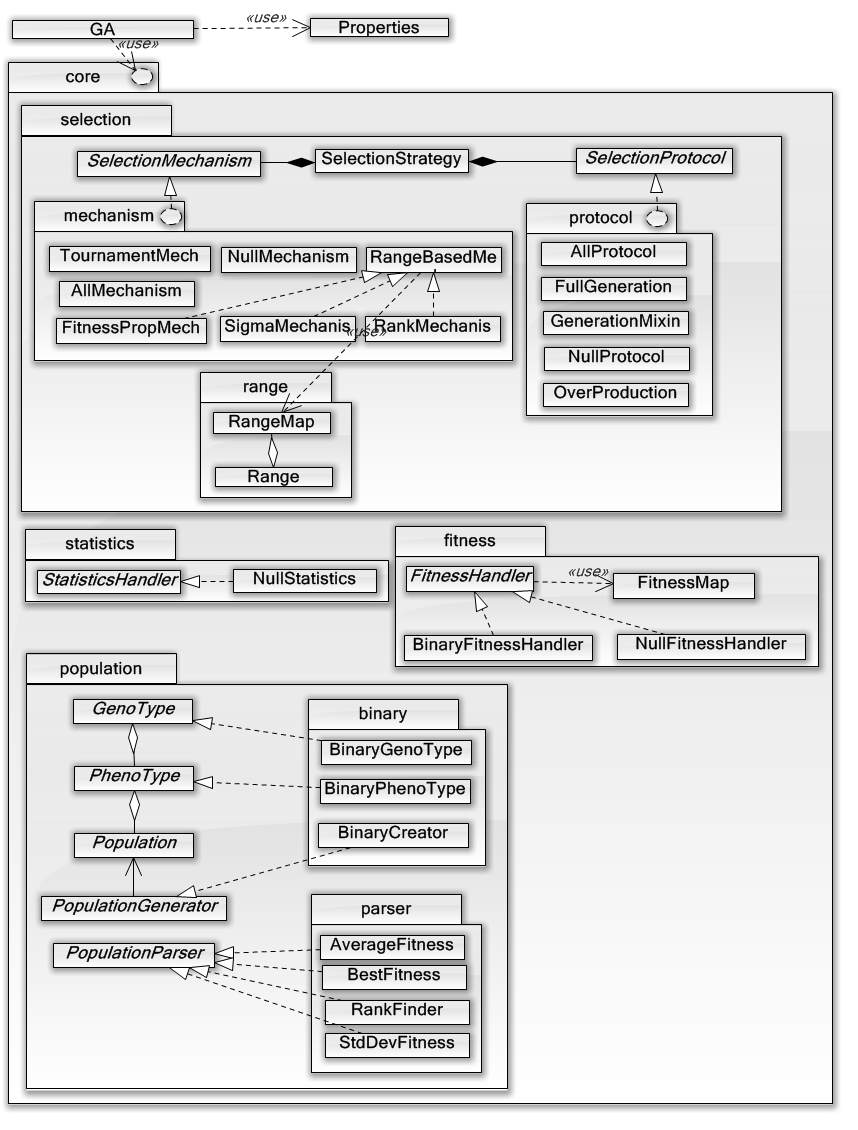
\includegraphics[width=.6\columnwidth]{./../images/GAStruct.png}}
				\caption{GA architecture}%
				\label{fig:gastruct}%
			\end{figure}

		\subsubsection{Problem specific}\label{sec:specific}
				In this exercise, we implement everything problem specific in a separate project. Our SpikeGenoType, SpikePhenoType, SpikeFitnessHandler and SpikePopulationCreator extends GenoType, PhenoType, FitnessHandler and PopulationGenerator from the core project respectivly.
		Our Spike project also implements an abstraction for the SpikeTrain, including functionality for different spike train distance metrics (waveform, spike time, spike interval), reading from file, and writing to file.
	\subsection{Genotype}\label{sec:geno}
		For the genotype representation we choose a discrete representation with cardinality $k~=~2$ and accuracy $acc$, which is decoded by the phenotype into the correct range based on which parameter the bit sequence is describing. The accuracy is an integer between 1 and 31, whihc determinds how many bits should be used to encode each parameter. The set of parameters for Izhikevich model each has it own range, described by $range_{param} \in [min_{param}, max_{param}]$. 
		\begin{align}
			range_a &\in [0.001, 0.2]\nonumber\\
			range_b &\in [0.01, 0.3]\nonumber\\
			range_c &\in [-80, -30]\nonumber\\
			range_d &\in [0.1, 10]\nonumber\\
			range_k &\in [0.01, 1.0]\nonumber
		\end{align}
		The conversion between the binary vector into real valued parameter is done by taking $acc$ bits and converting them to an integer $coef_{param}$. $subvector(bitvector, param)$ extracts the parameter relevant bits from the genotype bitvector.
		\begin{align}
			param &\in \{a, b, c, d, k\}\nonumber\\
			acc &= 8\nonumber\\
			bitvector &= 00001101\dots11100110\nonumber\\
			bitvector_{param} &= subvector(bitvector, param)\nonumber\\
			coef_{param} &= (bitvector_{param})_{10}\nonumber\\
			step_{param} &= (max_{param}-min_{param})/2^{acc}\nonumber\\
			param &= min_{param}+(coef_{param}*step_{param})\nonumber
		\end{align}
	\subsection{Fitness function}\label{sec:fitness}
		Our fitness function is based on the different SDM's implemented during this project, where $F_j$ is the phenotype in question, and $E_j$ the error found by the SDM associated with $F_j$.
		\begin{align}
			Fitness(F_j) &= \frac{1}{1+E_j}\nonumber
		\end{align}
\section{Test cases}\label{sec:test}
	Intro
	\subsection{Izzy 1}
		\subsubsection{Spike time distance metric}
			\begin{figure}[H]
				\centering
					\begin{subfigure}{.5\textwidth}
						\centering
						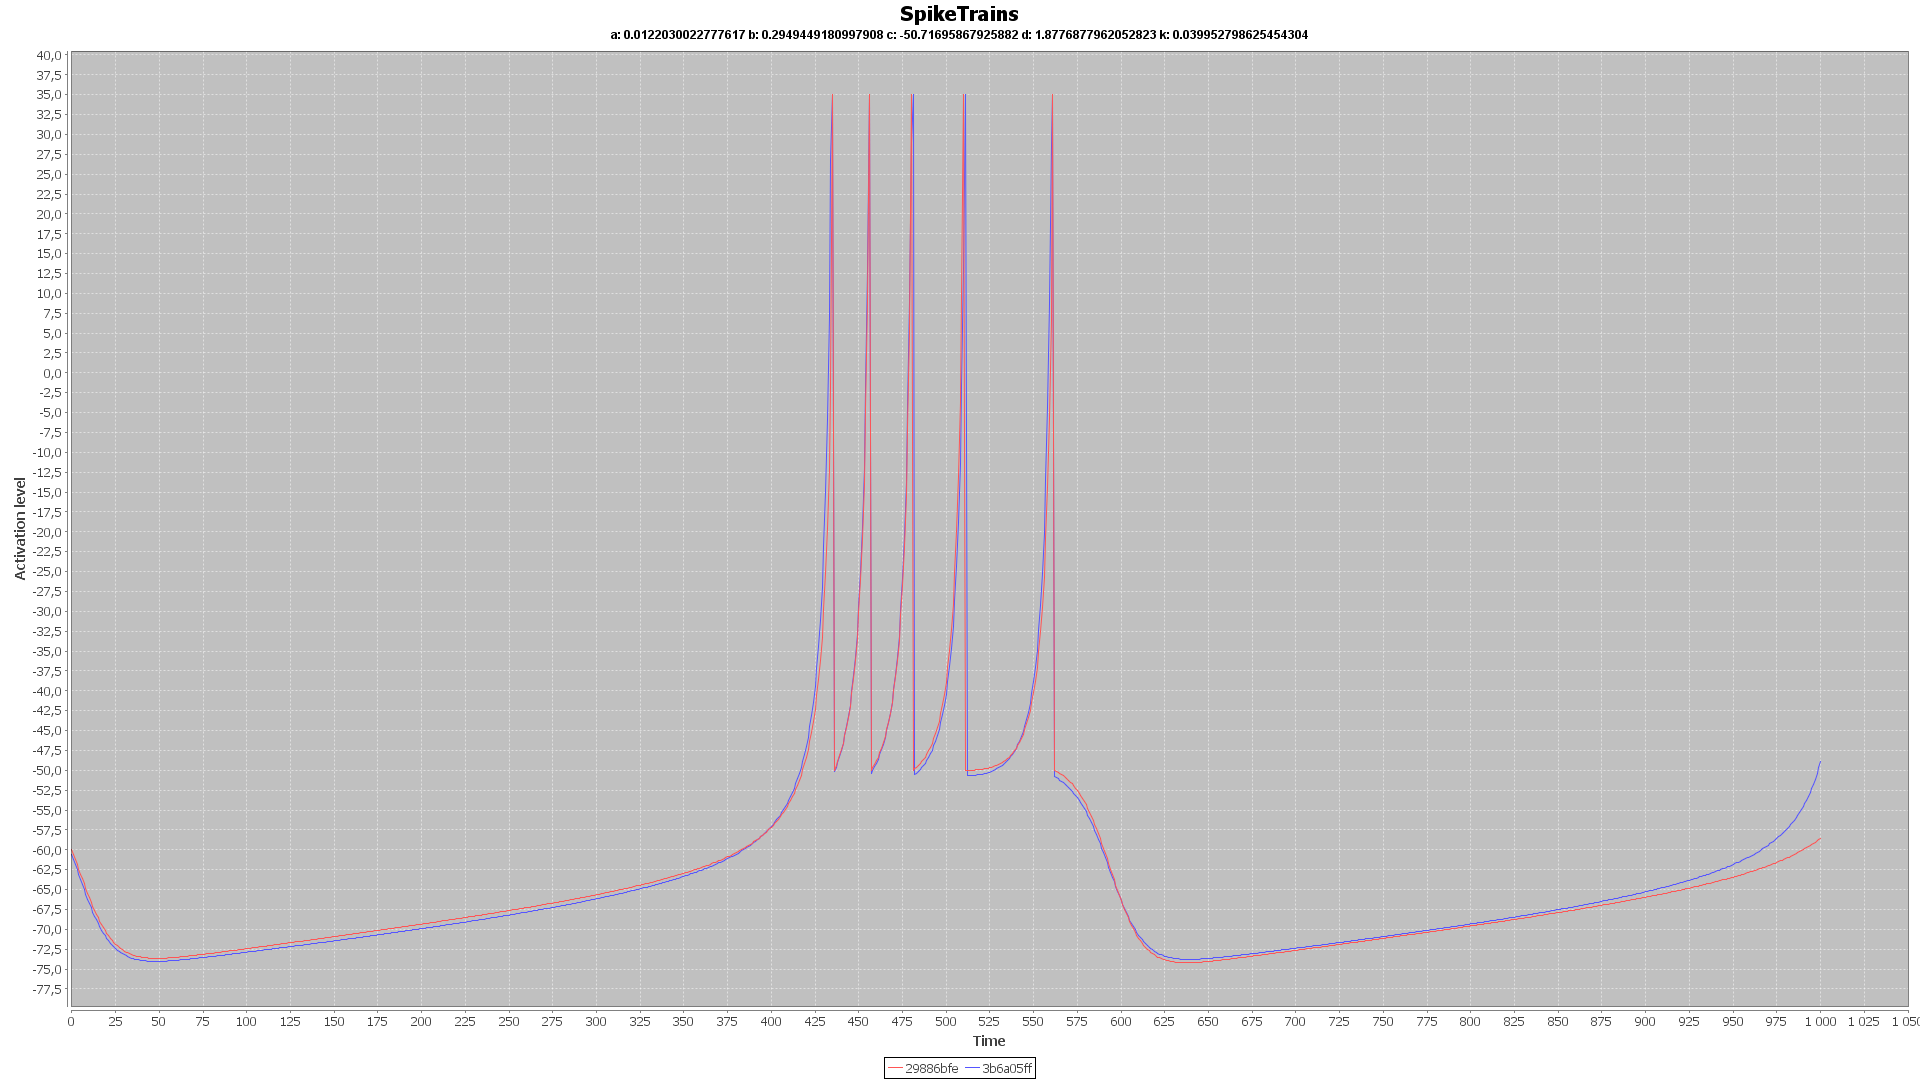
\includegraphics[width=\linewidth]{./../images/izzy1/time/plot.png}
						
						\label{fig:sub1a}
					\end{subfigure}%
					\begin{subfigure}{.5\textwidth}
						\centering
						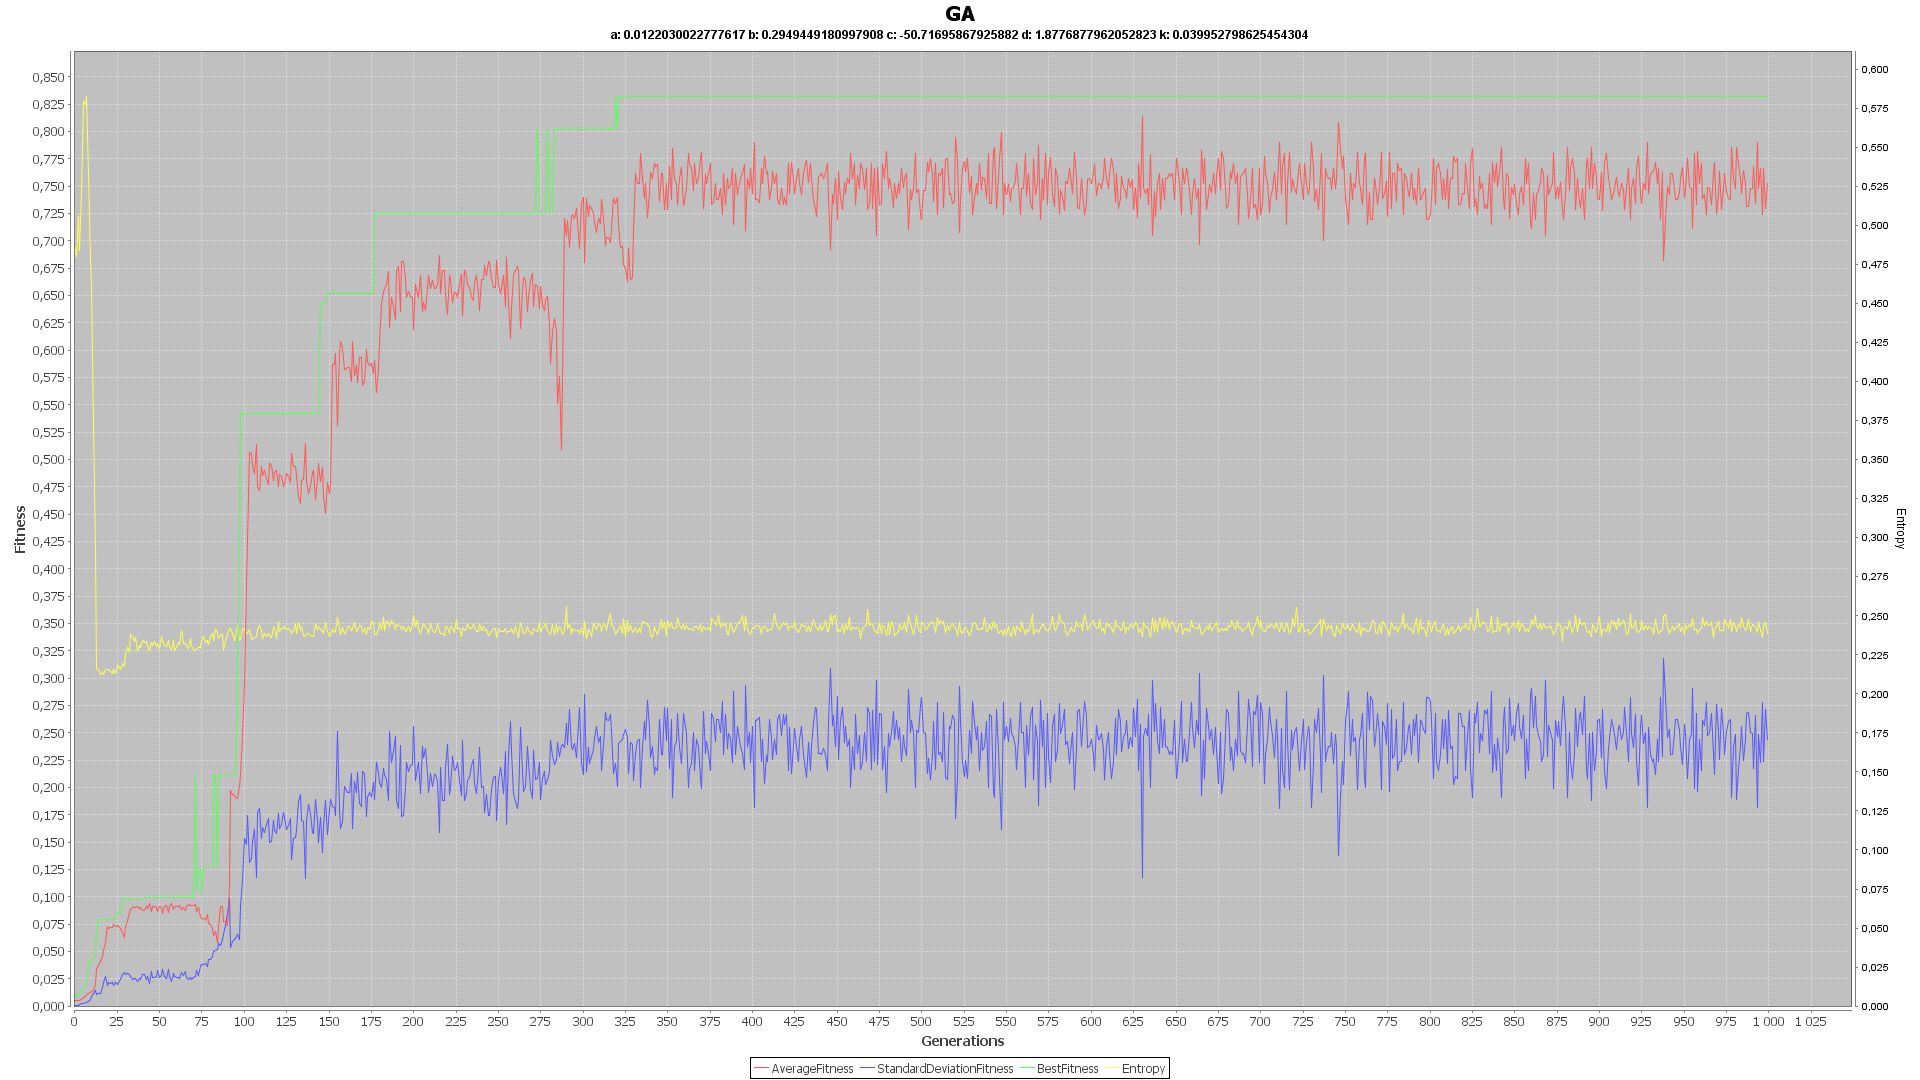
\includegraphics[width=\linewidth]{./../images/izzy1/time/prog.png}
						
						\label{fig:sub1b}
					\end{subfigure}
					
					\label{fig:plot1}
			\end{figure}
			
		\subsubsection{Spike interval distance metric}
			\begin{figure}[H]
				\centering
					\begin{subfigure}{.5\textwidth}
						\centering
						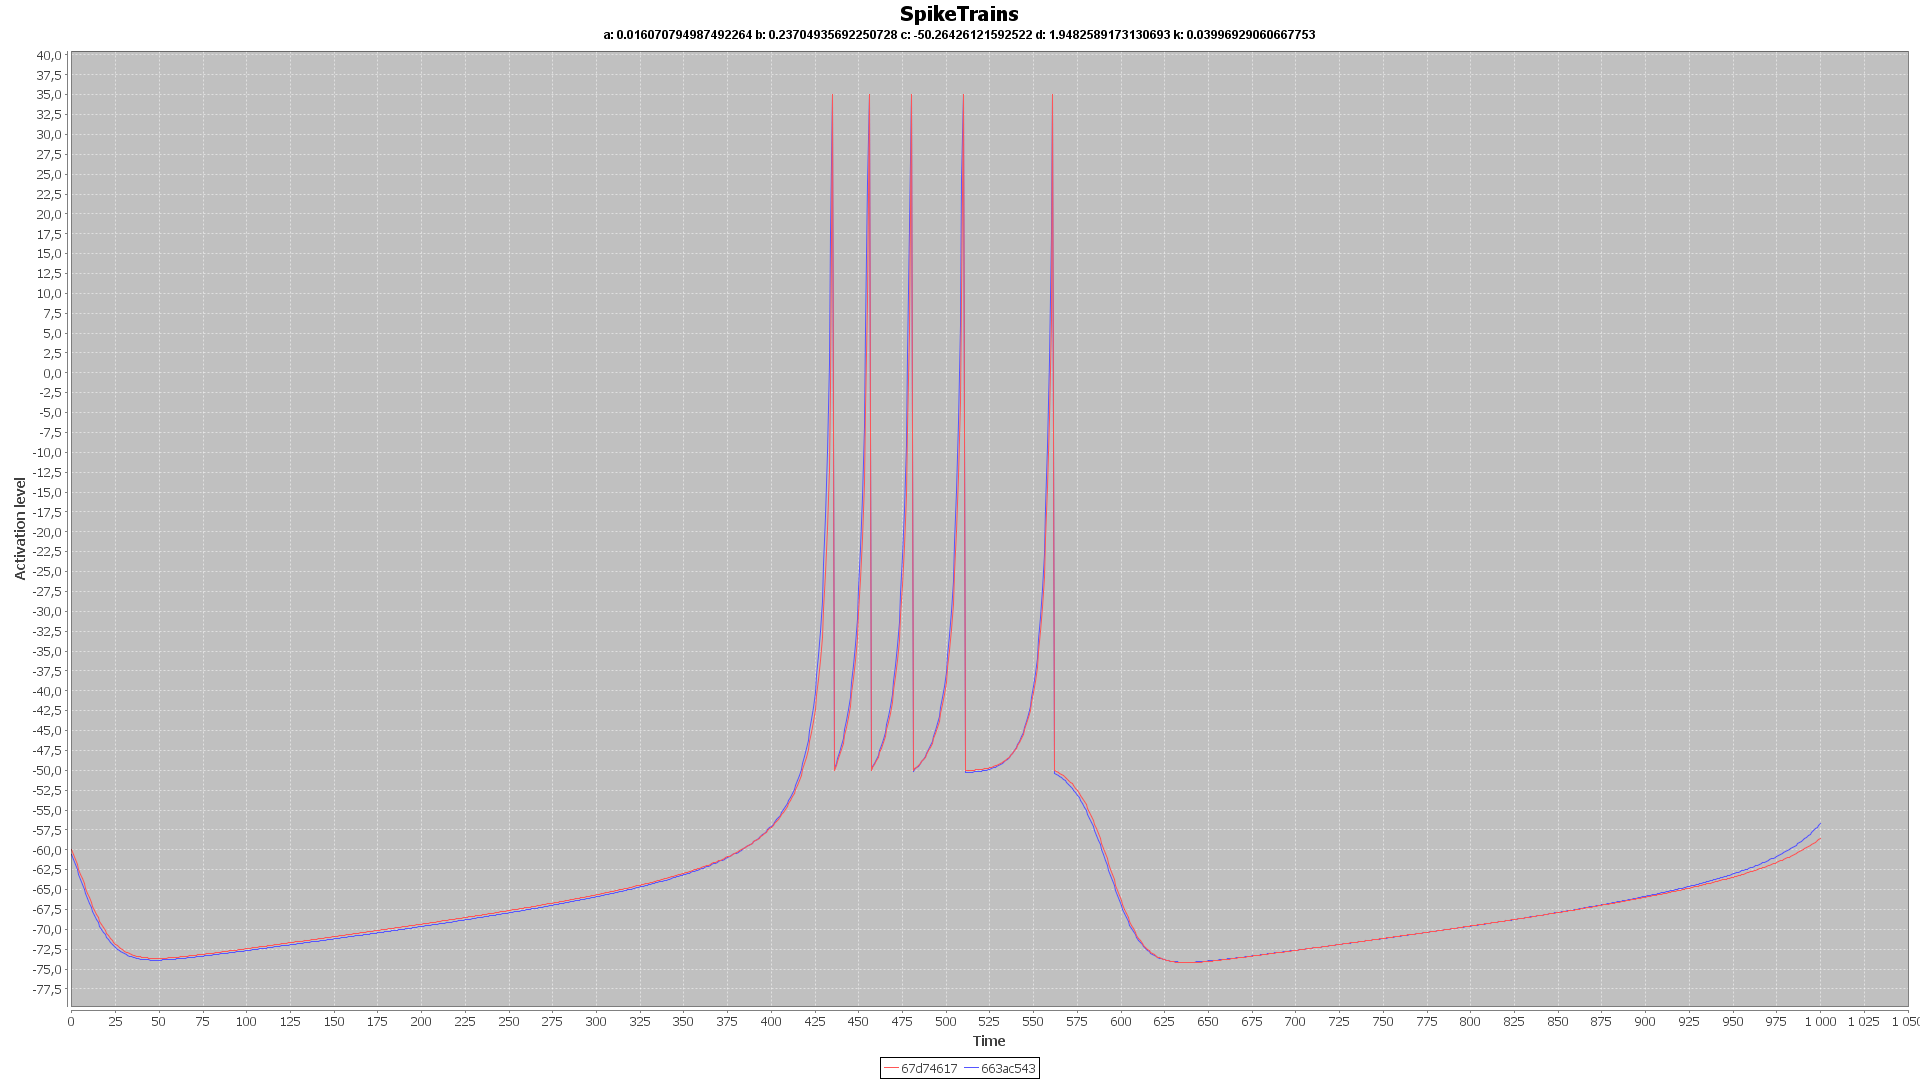
\includegraphics[width=\linewidth]{./../images/izzy1/interval/plot.png}
						
						\label{fig:sub2a}
					\end{subfigure}%
					\begin{subfigure}{.5\textwidth}
						\centering
						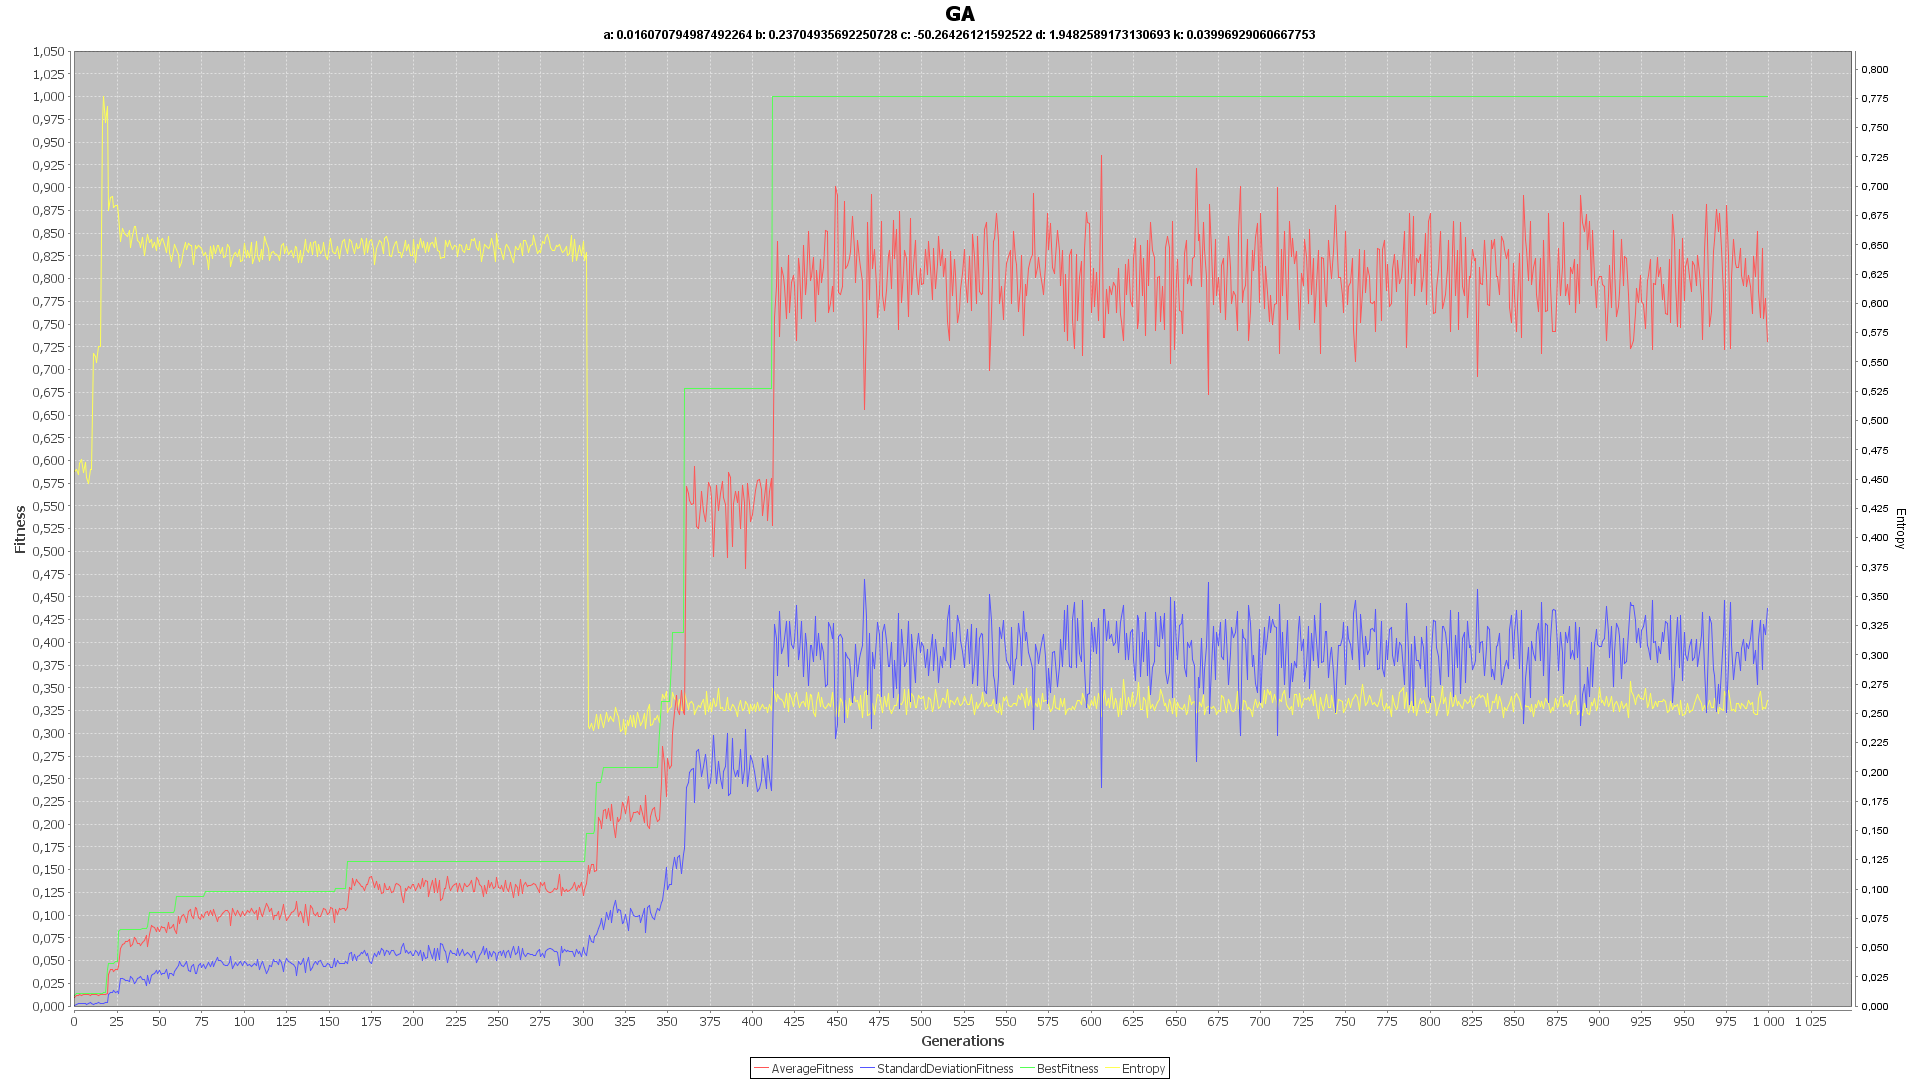
\includegraphics[width=\linewidth]{./../images/izzy1/interval/prog.png}
						
						\label{fig:sub2b}
					\end{subfigure}
					
					\label{fig:plot2}
			\end{figure}
		
		\subsubsection{Waveform distance metric}
		
	\subsection{Izzy 2}
		\subsubsection{Spike time distance metric}
			\begin{figure}[H]
				\centering
					\begin{subfigure}{.5\textwidth}
						\centering
						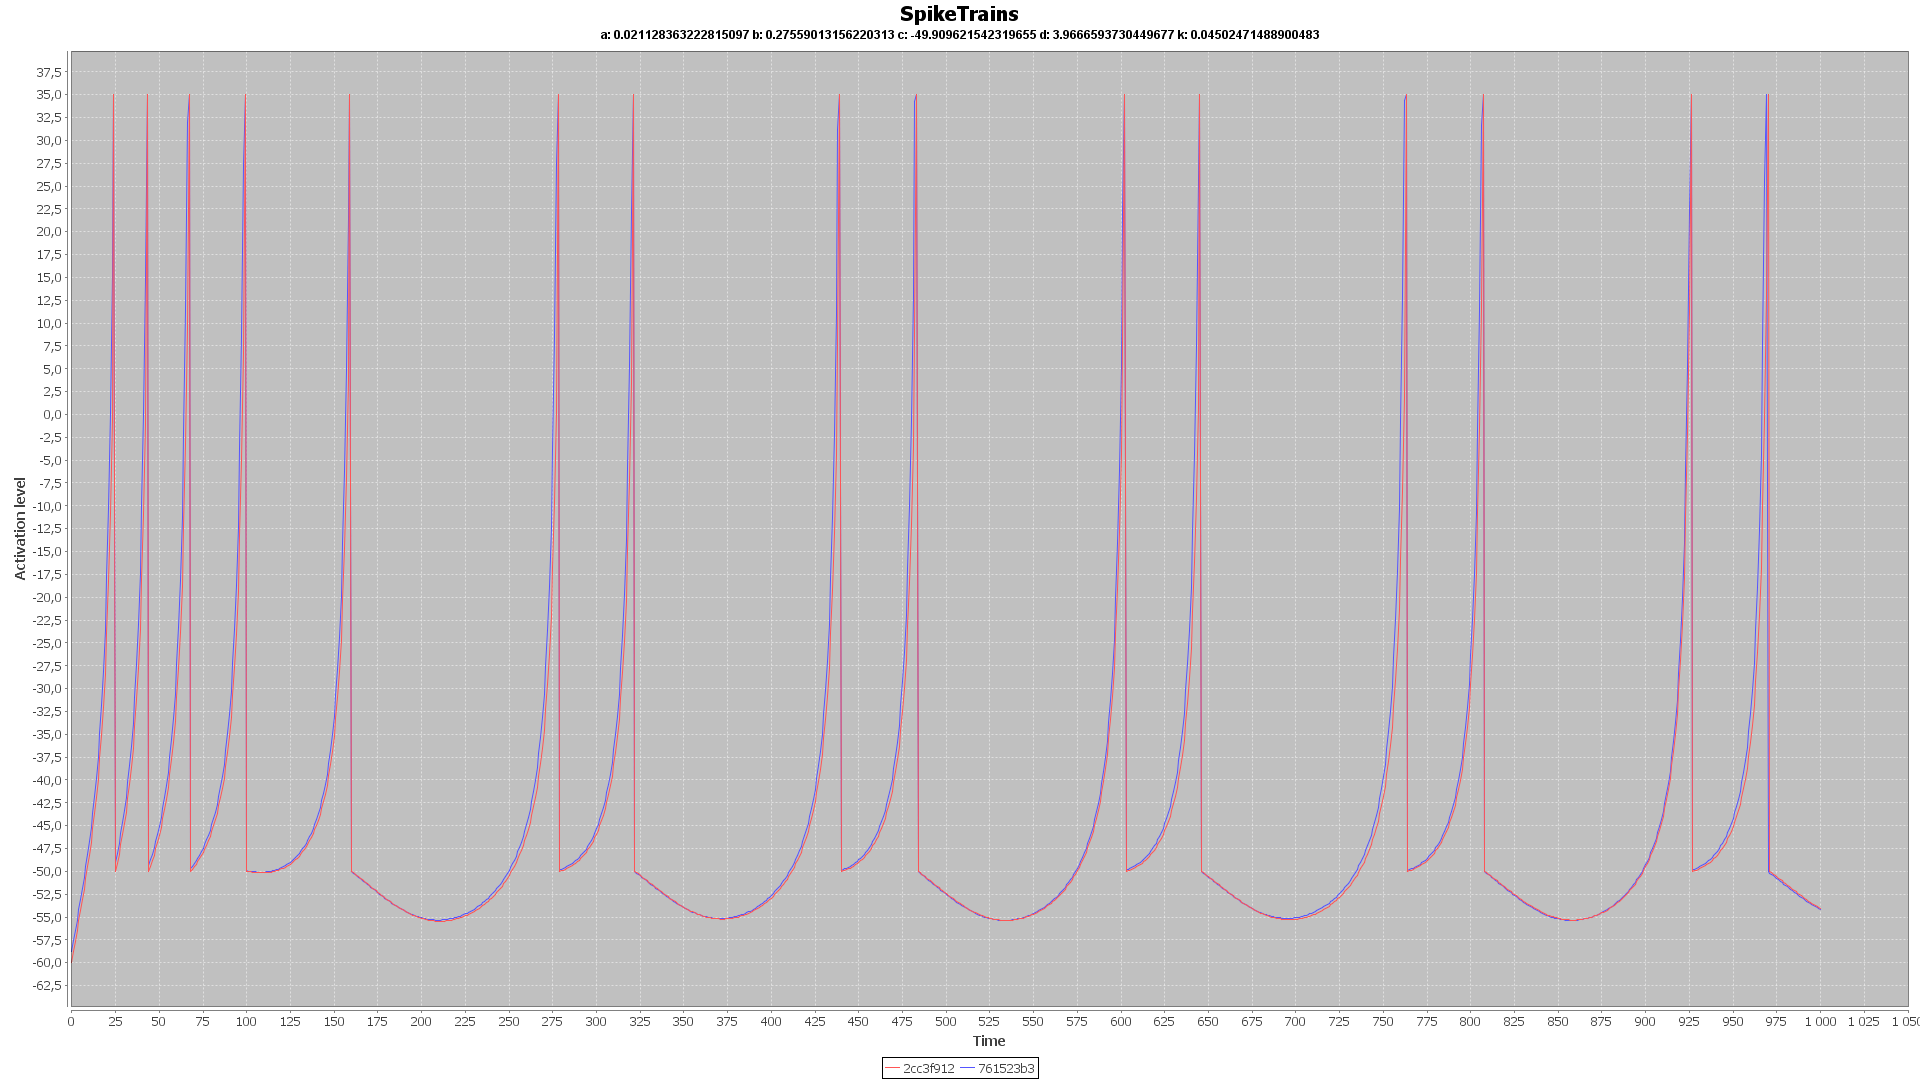
\includegraphics[width=\linewidth]{./../images/izzy2/time/plot.png}
						
						\label{fig:sub4a}
					\end{subfigure}%
					\begin{subfigure}{.5\textwidth}
						\centering
						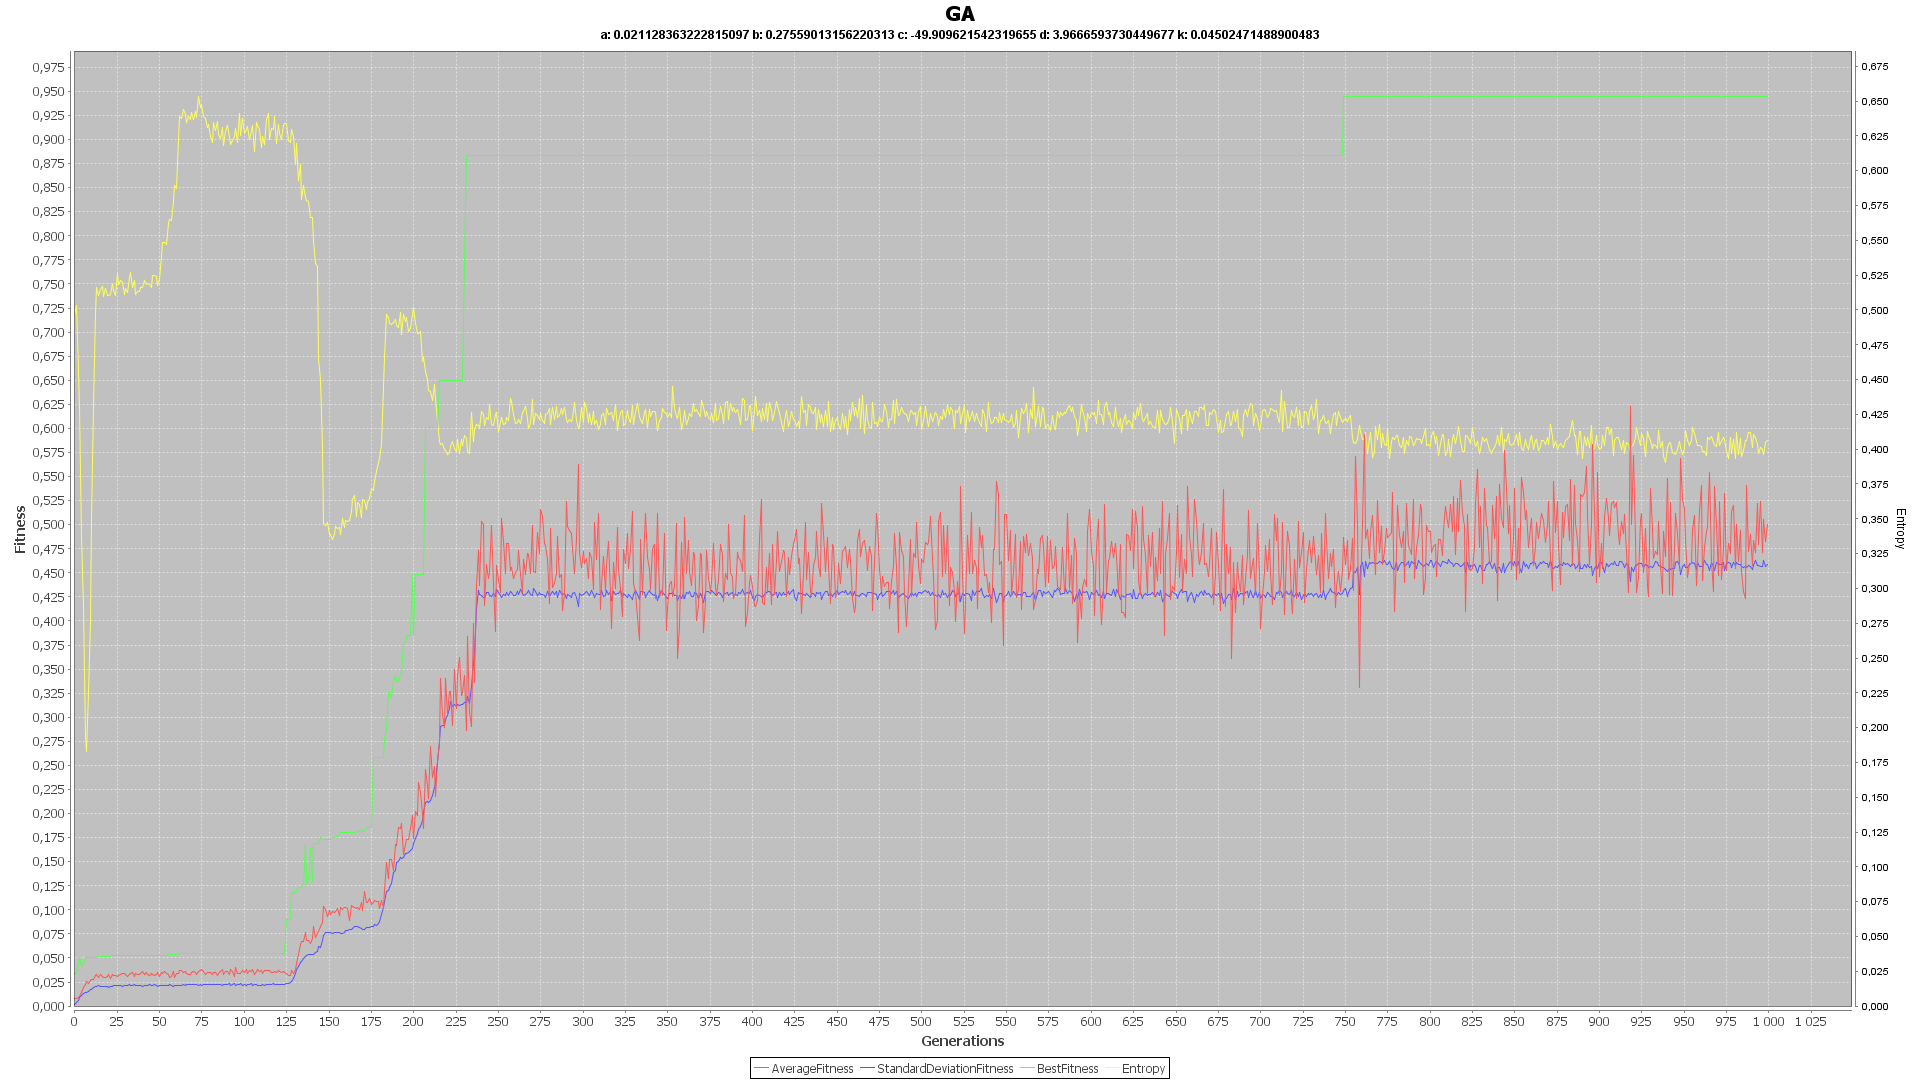
\includegraphics[width=\linewidth]{./../images/izzy2/time/prog.png}
						
						\label{fig:sub4b}
					\end{subfigure}
					
					\label{fig:plot4}
			\end{figure}
			
		\subsubsection{Spike interval distance metric}
			\begin{figure}[H]
				\centering
					\begin{subfigure}{.5\textwidth}
						\centering
						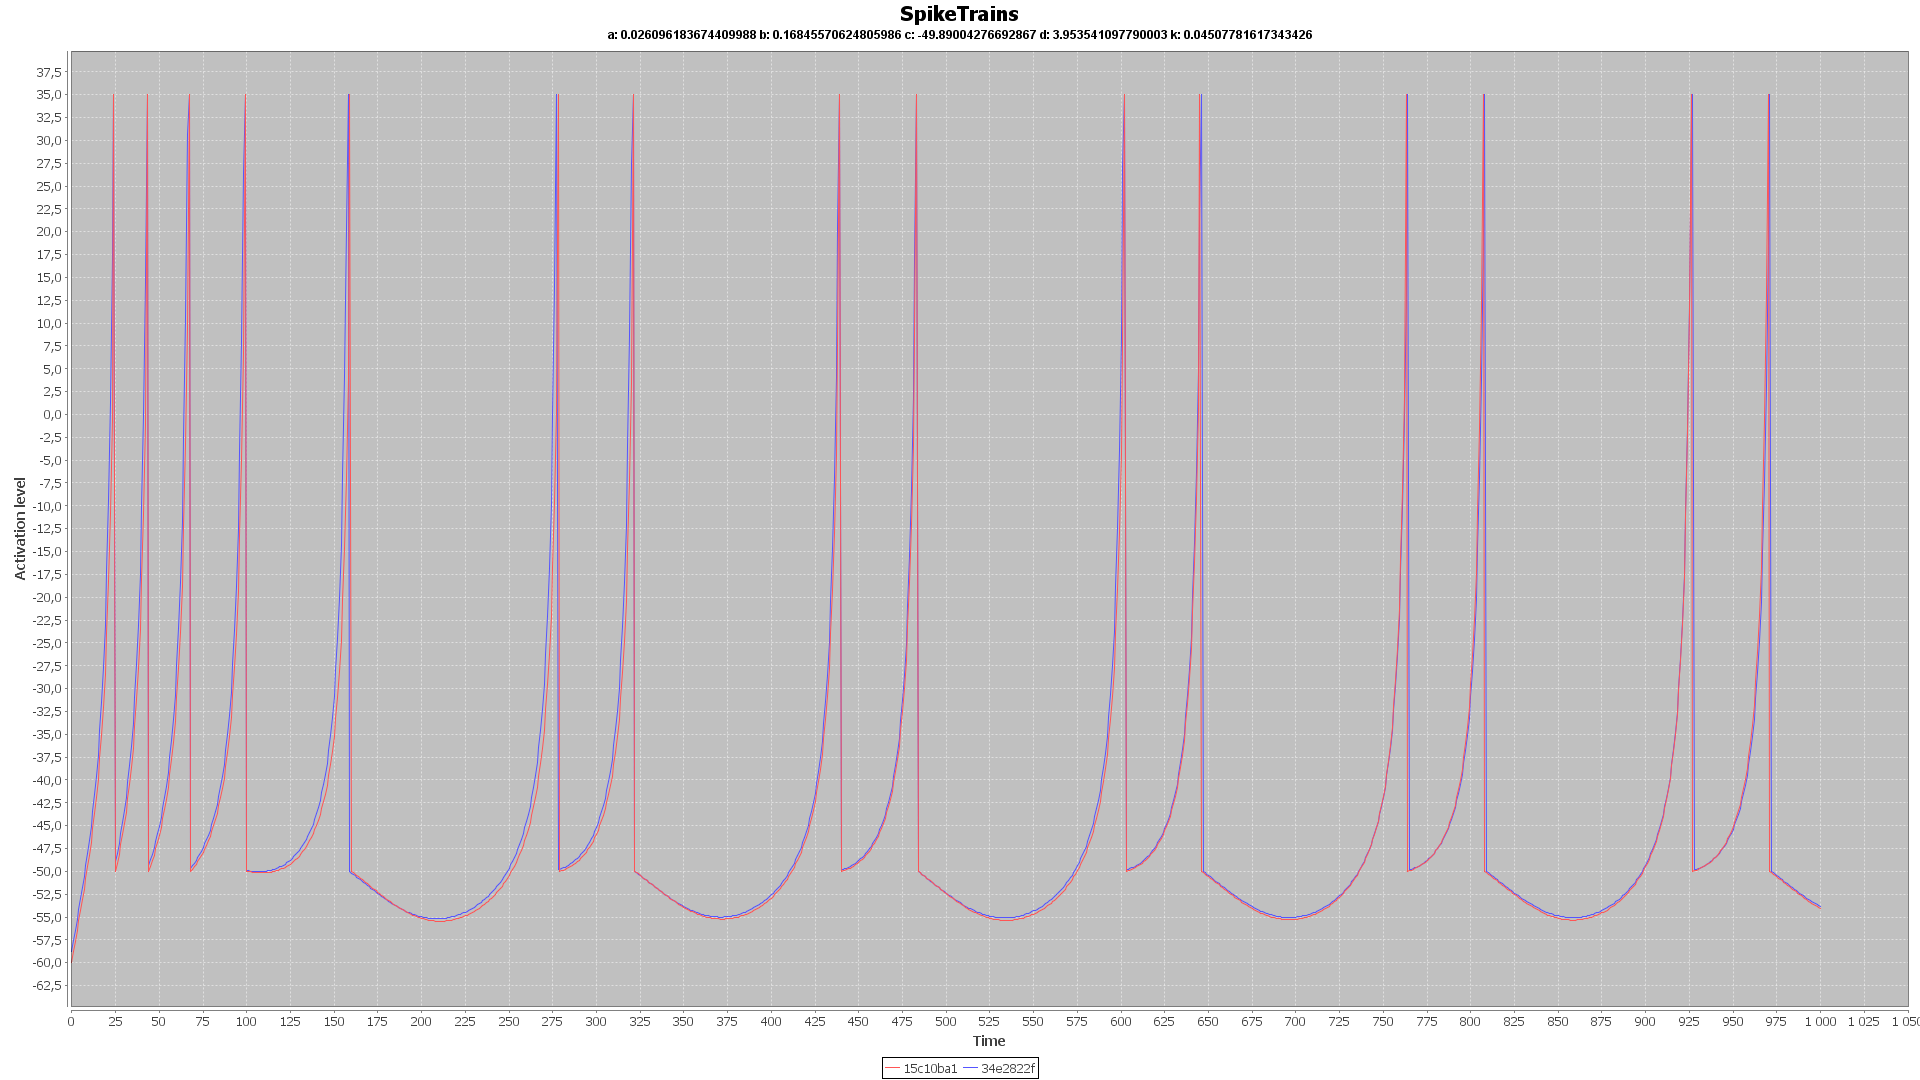
\includegraphics[width=\linewidth]{./../images/izzy2/interval/plot.png}
						
						\label{fig:sub5a}
					\end{subfigure}%
					\begin{subfigure}{.5\textwidth}
						\centering
						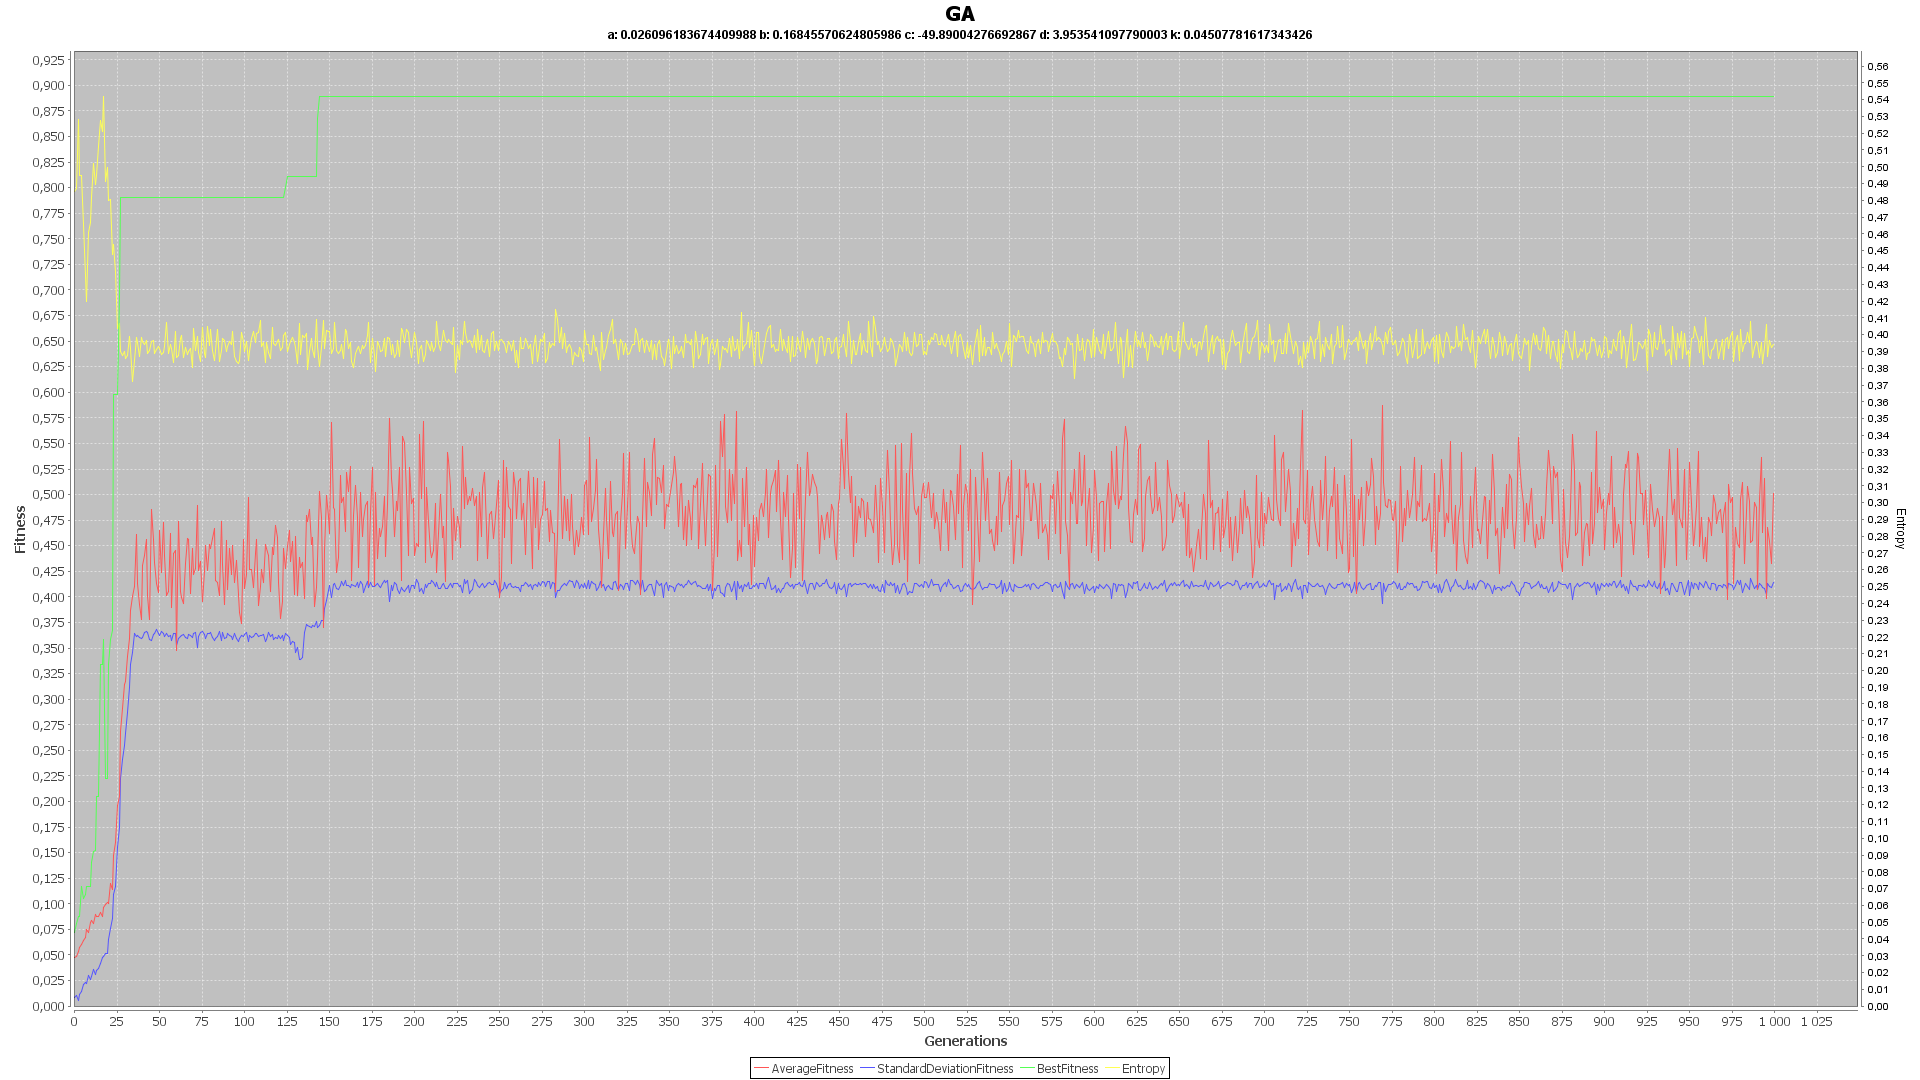
\includegraphics[width=\linewidth]{./../images/izzy2/interval/prog.png}
						
						\label{fig:sub5b}
					\end{subfigure}
					
					\label{fig:plot5}
			\end{figure}
			
		\subsubsection{Waveform distance metric}
		
	\subsection{Izzy 3}
		\subsubsection{Spike time distance metric}
			\begin{figure}[H]
				\centering
					\begin{subfigure}{.5\textwidth}
						\centering
						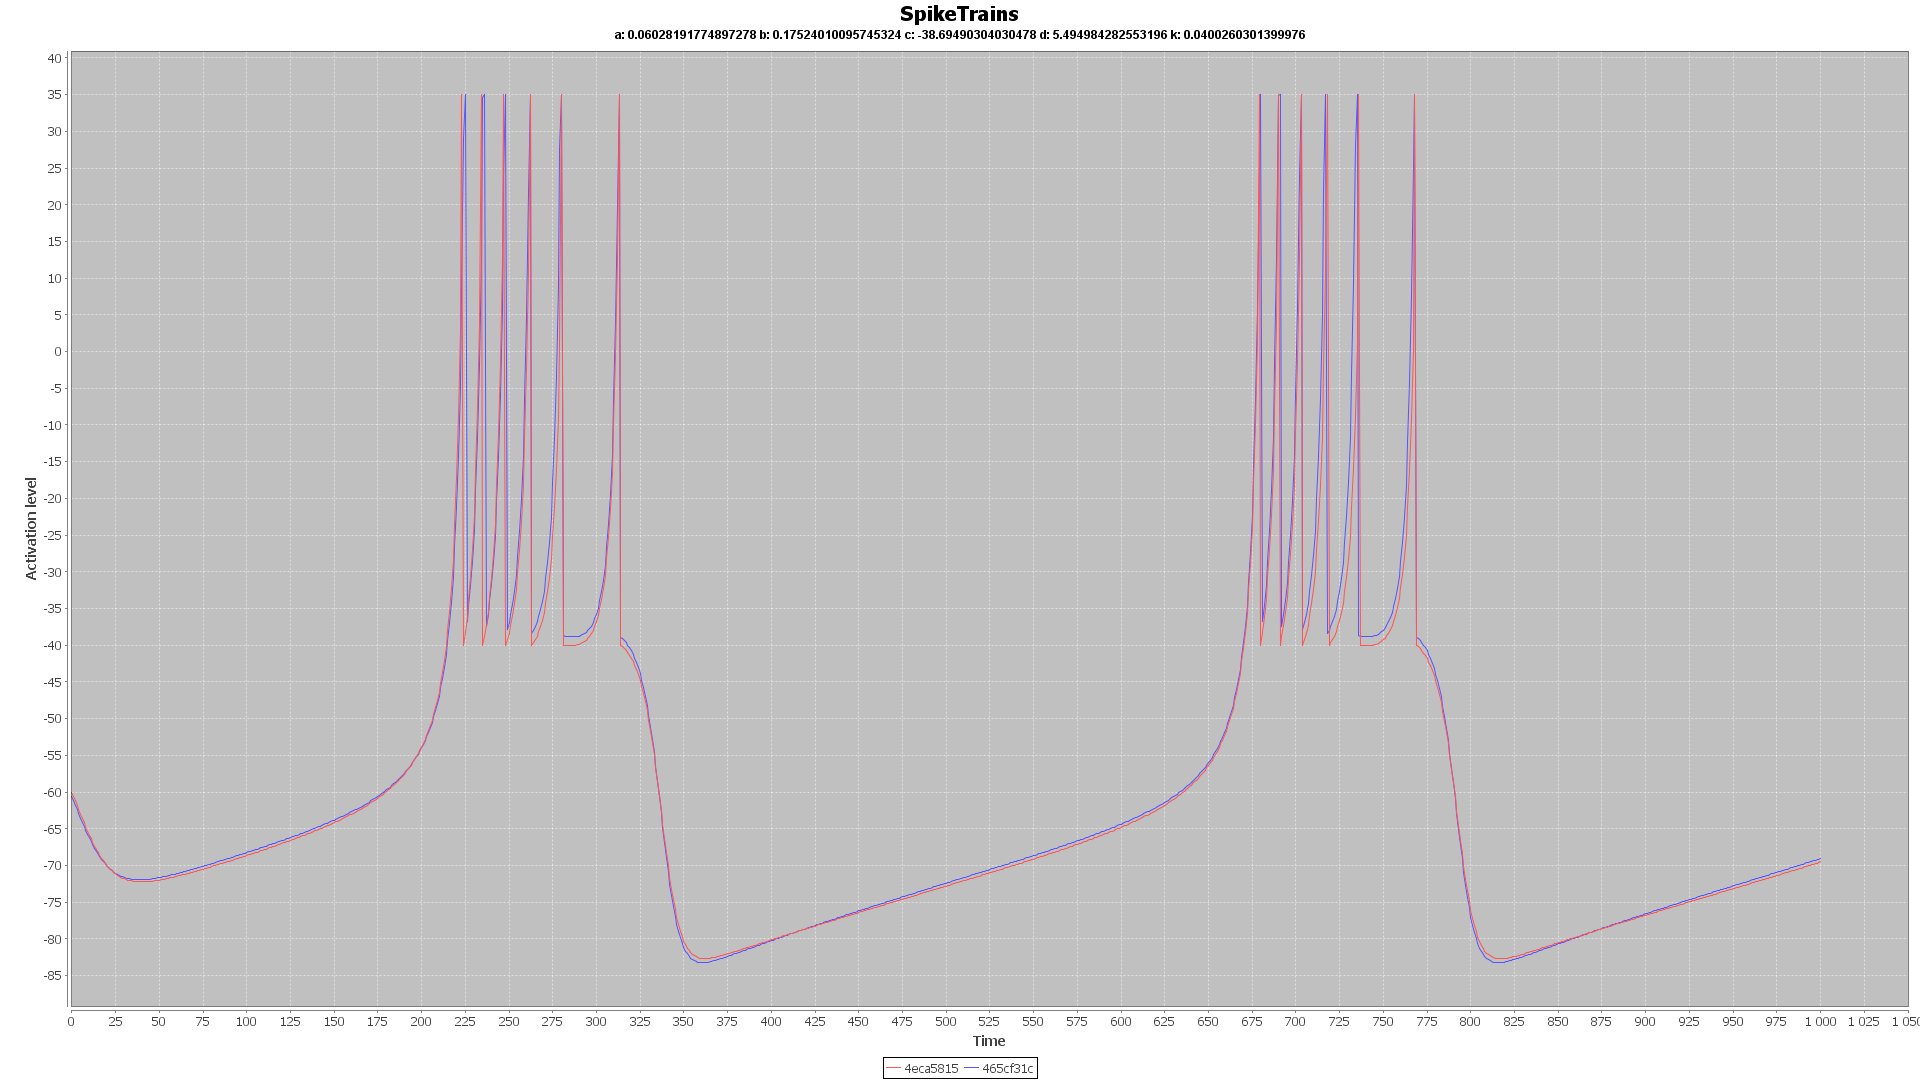
\includegraphics[width=\linewidth]{./../images/izzy3/time/plot.png}
						
						\label{fig:sub7a}
					\end{subfigure}%
					\begin{subfigure}{.5\textwidth}
						\centering
						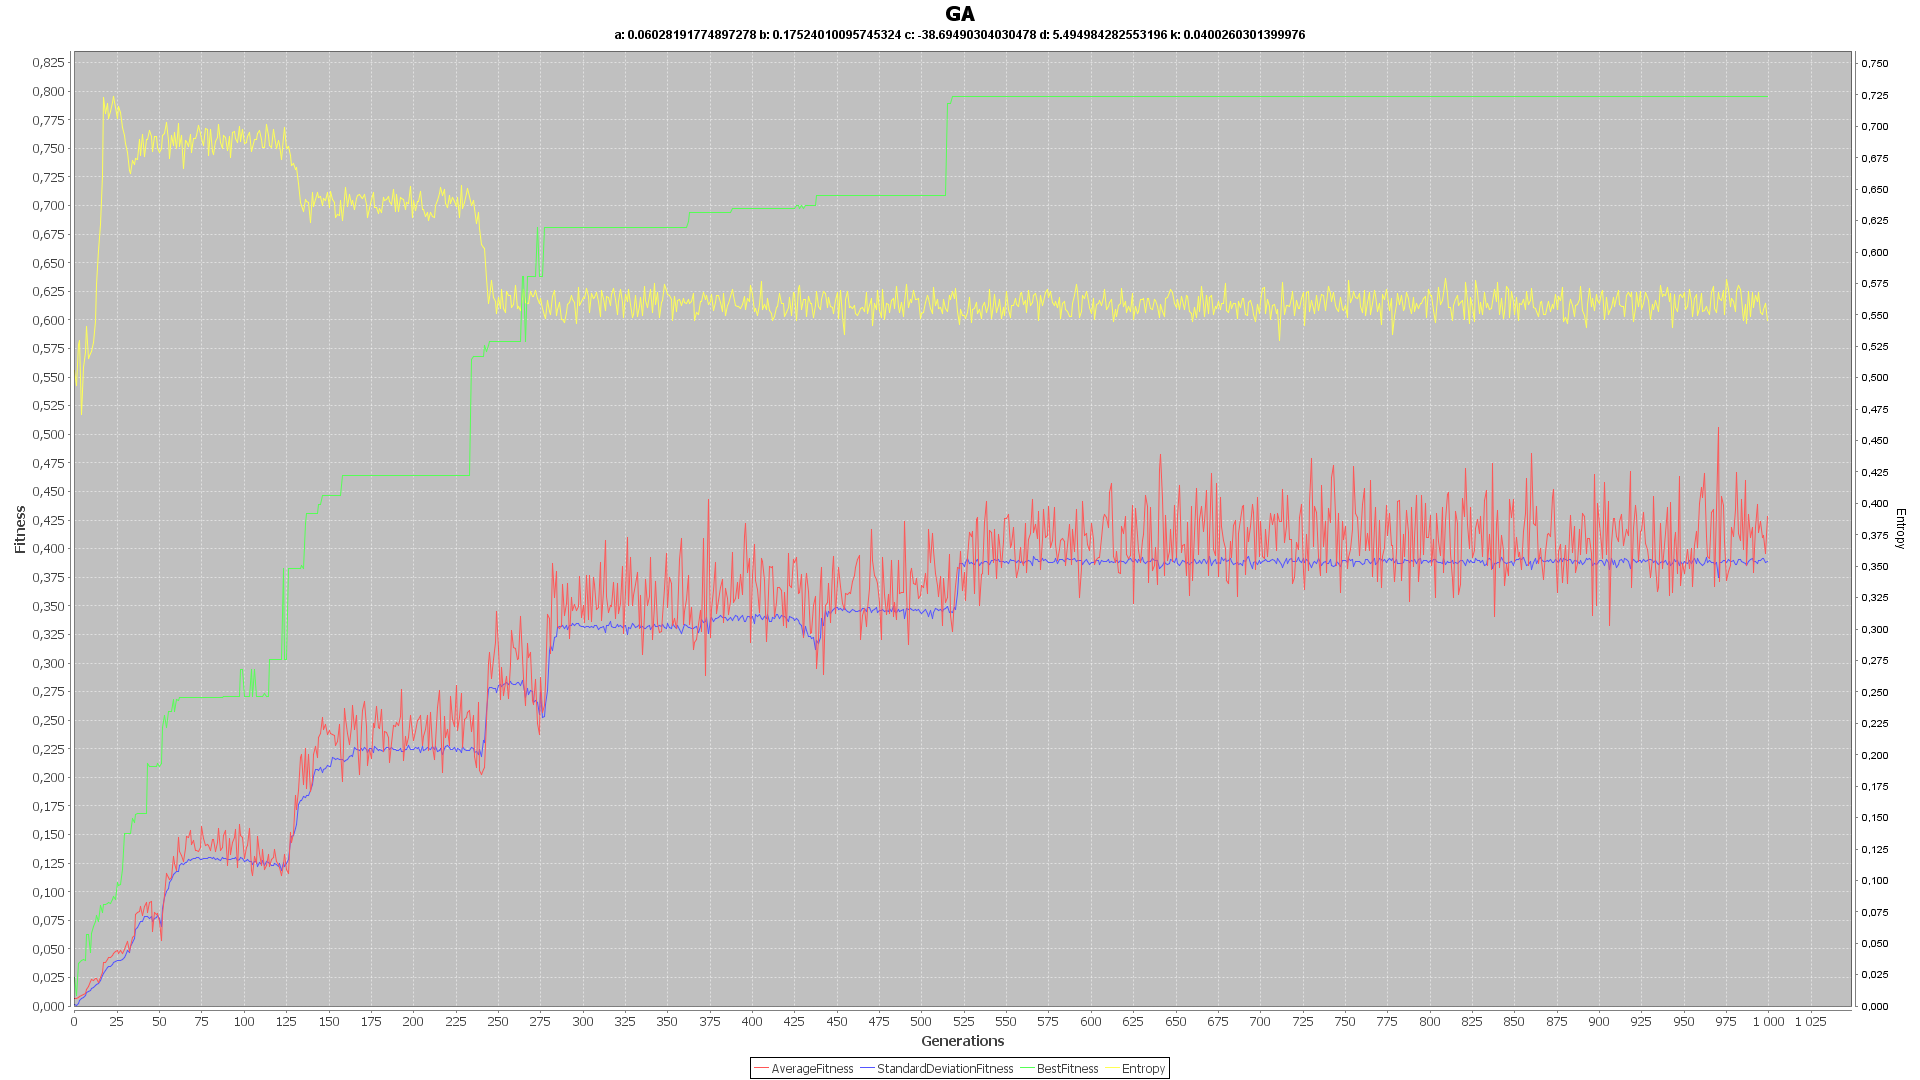
\includegraphics[width=\linewidth]{./../images/izzy3/time/prog.png}
						
						\label{fig:sub7b}
					\end{subfigure}
					
					\label{fig:plot7}
			\end{figure}
			
		\subsubsection{Spike interval distance metric}
			\begin{figure}[H]
				\centering
					\begin{subfigure}{.5\textwidth}
						\centering
						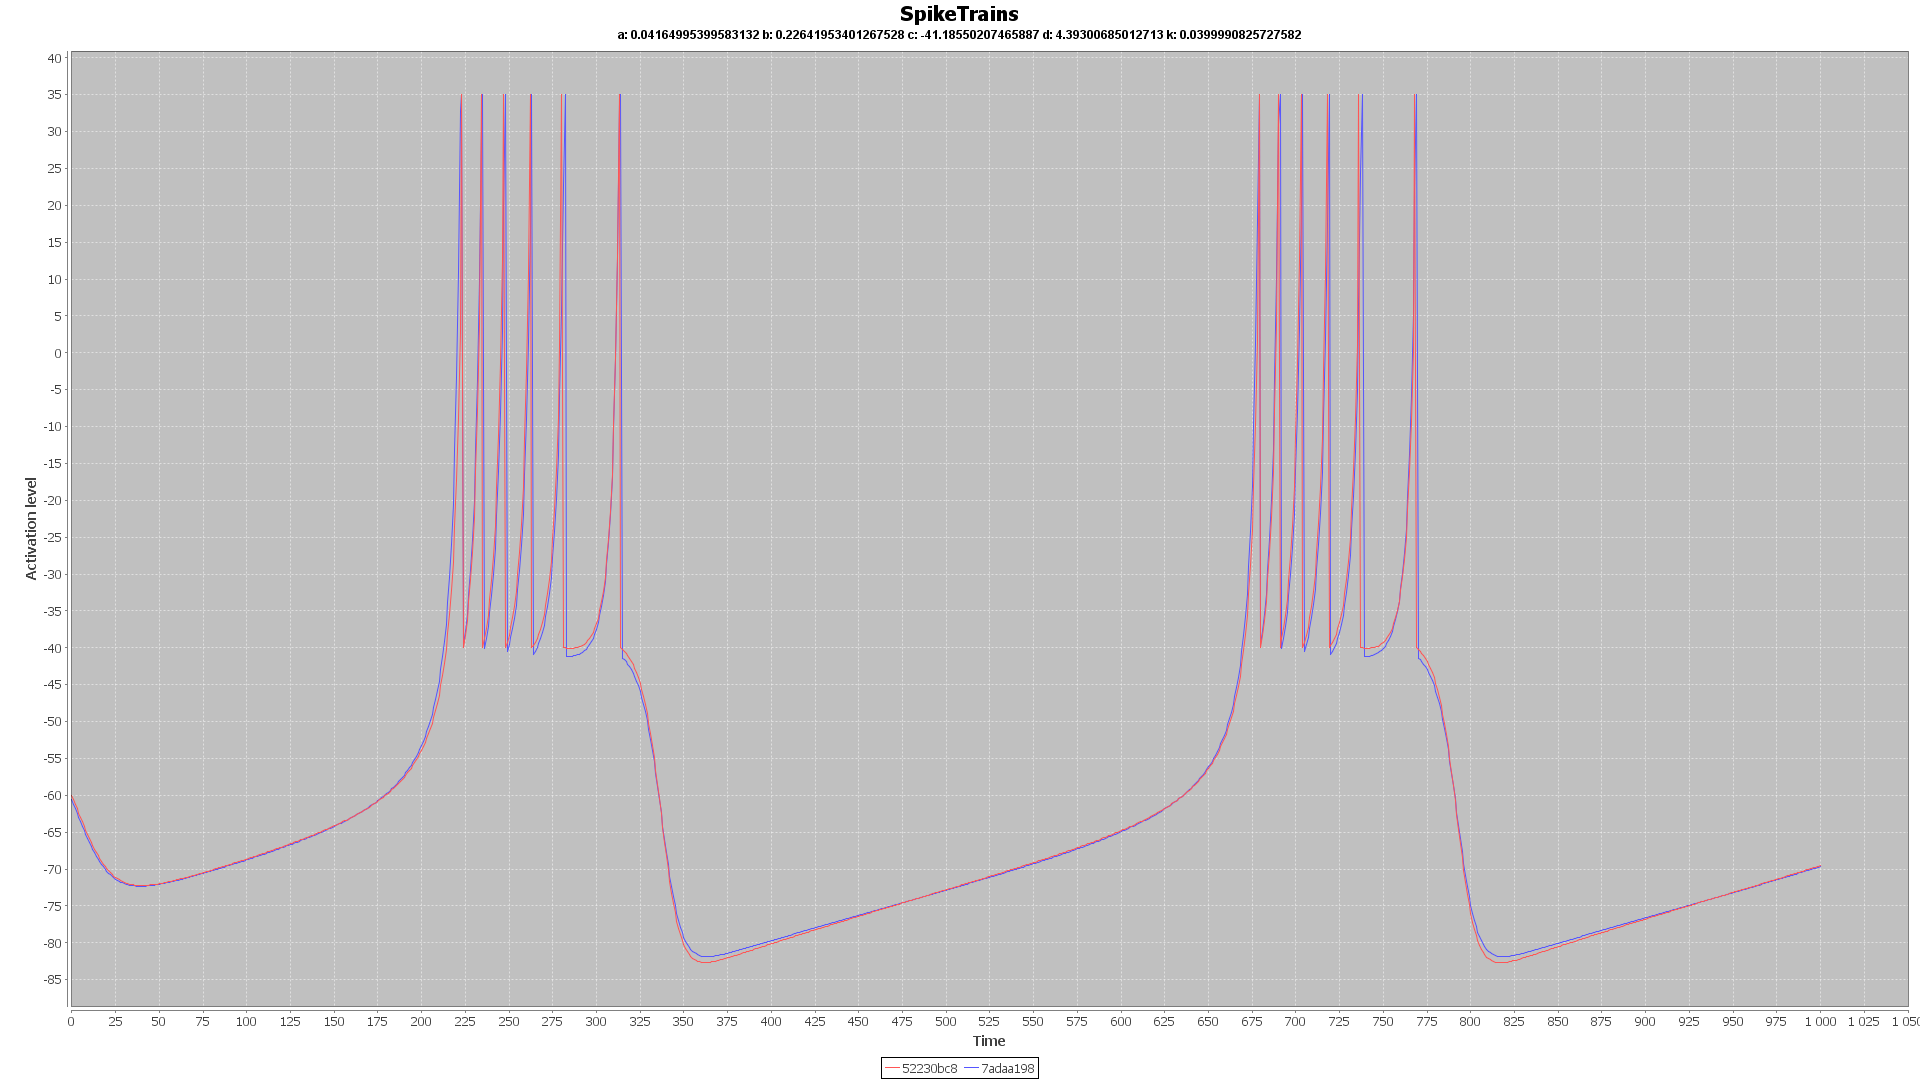
\includegraphics[width=\linewidth]{./../images/izzy3/interval/plot.png}
						
						\label{fig:sub8a}
					\end{subfigure}%
					\begin{subfigure}{.5\textwidth}
						\centering
						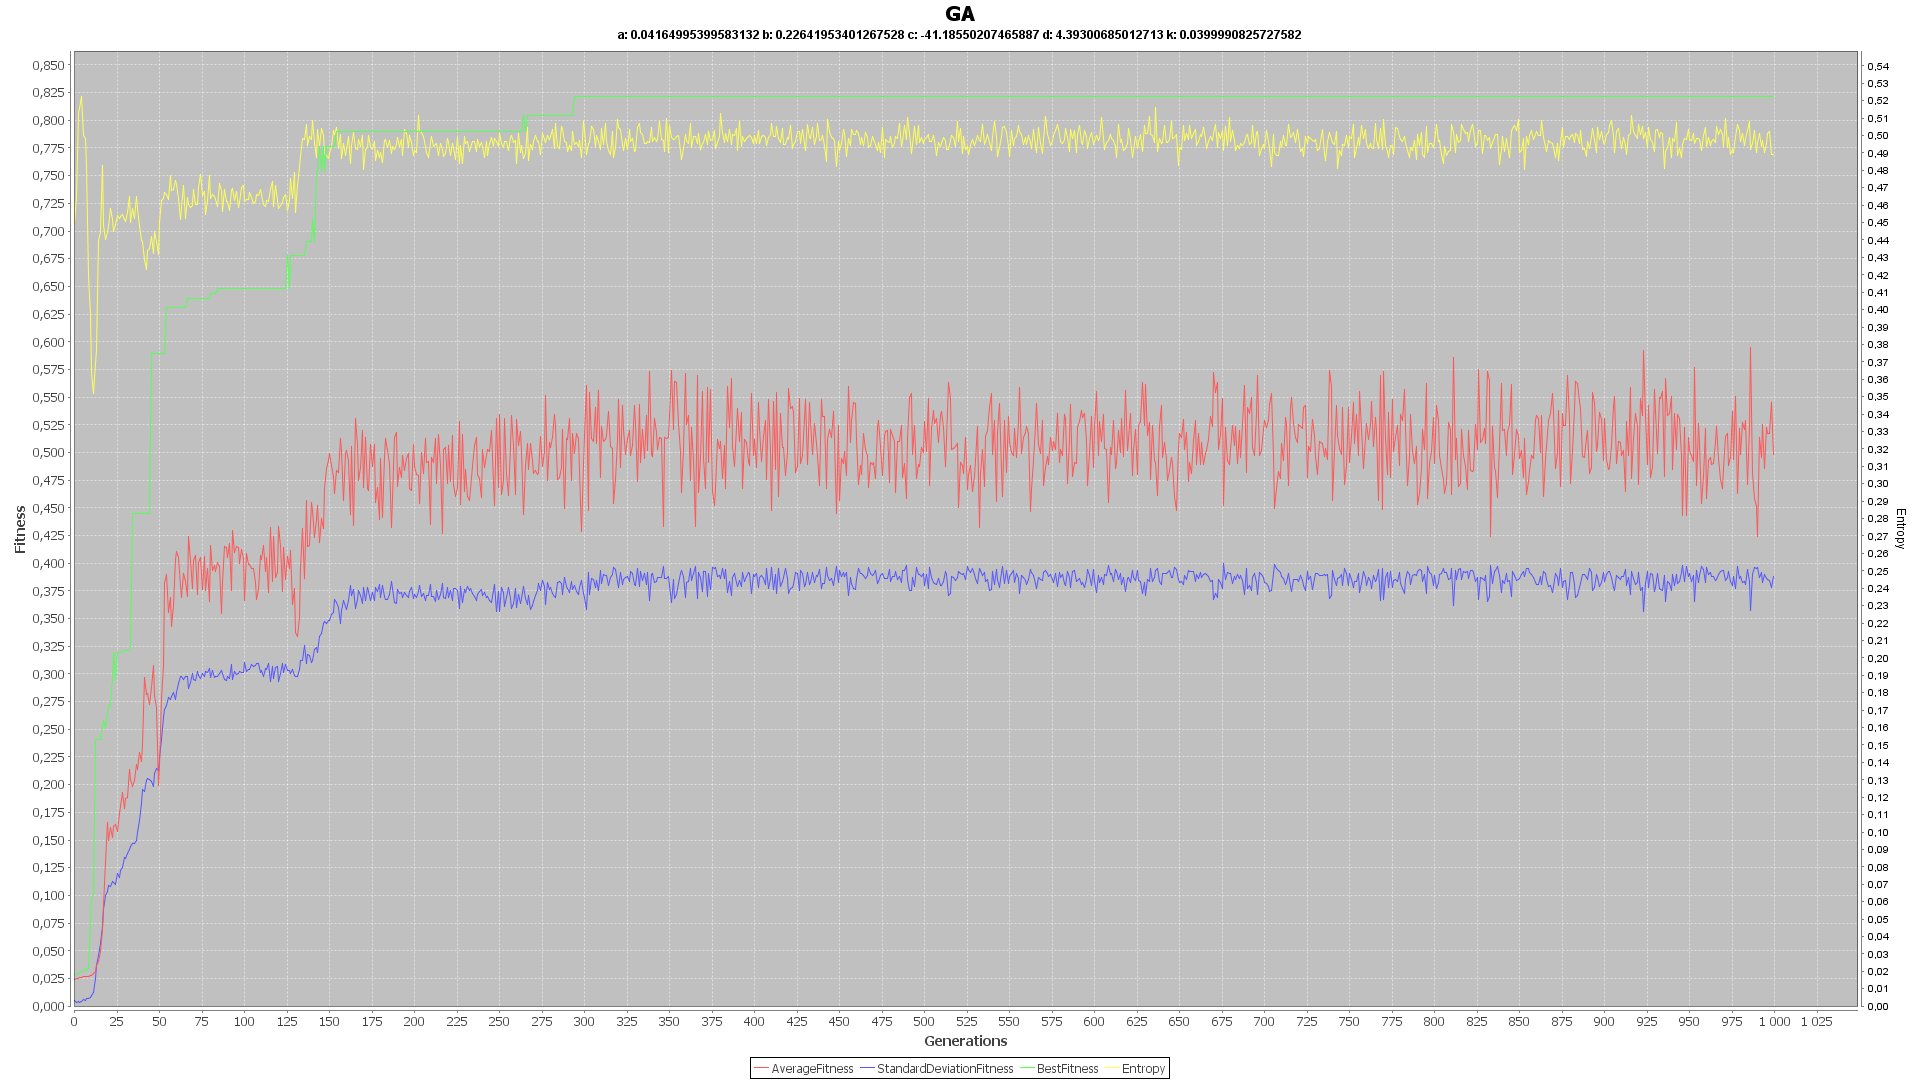
\includegraphics[width=\linewidth]{./../images/izzy3/interval/prog.png}
						
						\label{fig:sub8b}
					\end{subfigure}
					
					\label{fig:test}
			\end{figure}
			
		\subsubsection{Waveform distance metric}
		
	\subsection{Izzy 4}
		\subsubsection{Spike time distance metric}
			\begin{figure}[H]
				\centering
					\begin{subfigure}{.5\textwidth}
						\centering
						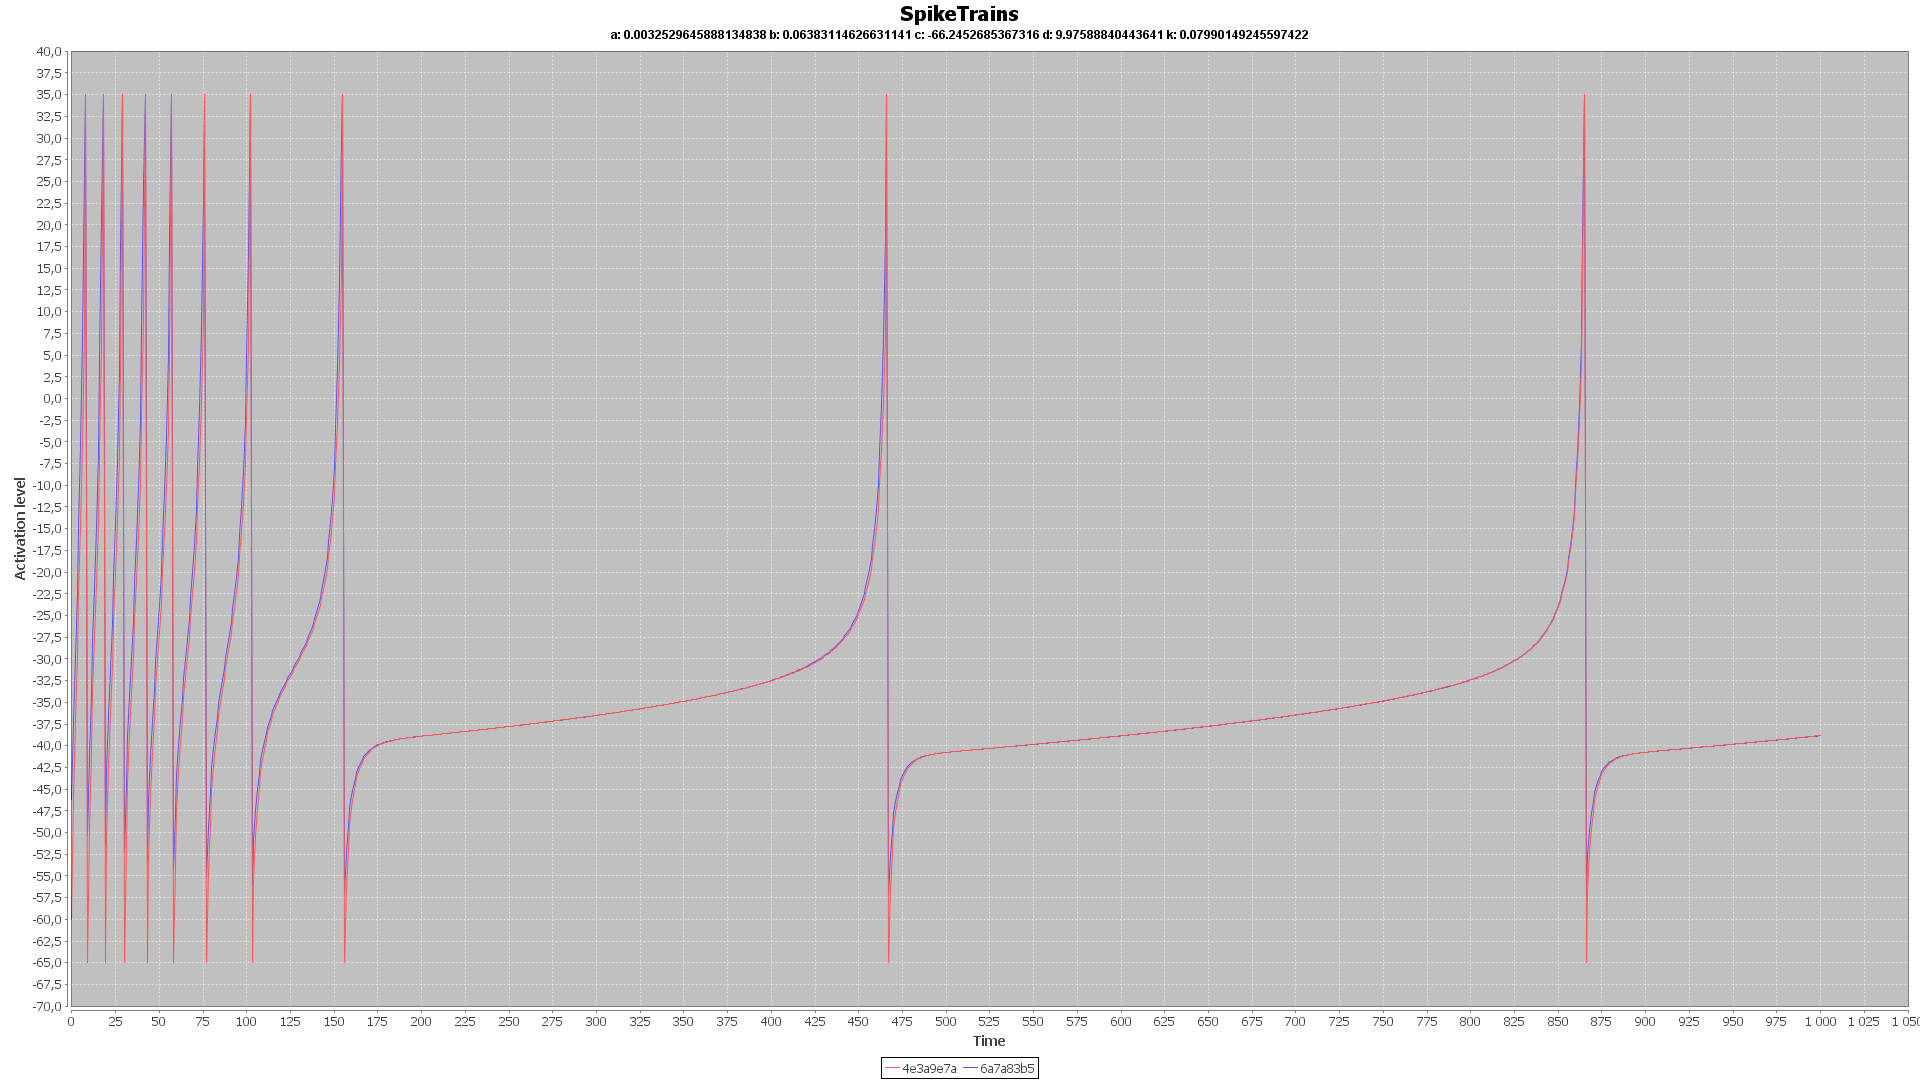
\includegraphics[width=\linewidth]{./../images/izzy4/time/plot.png}
						
						\label{fig:sub10a}
					\end{subfigure}%
					\begin{subfigure}{.5\textwidth}
						\centering
						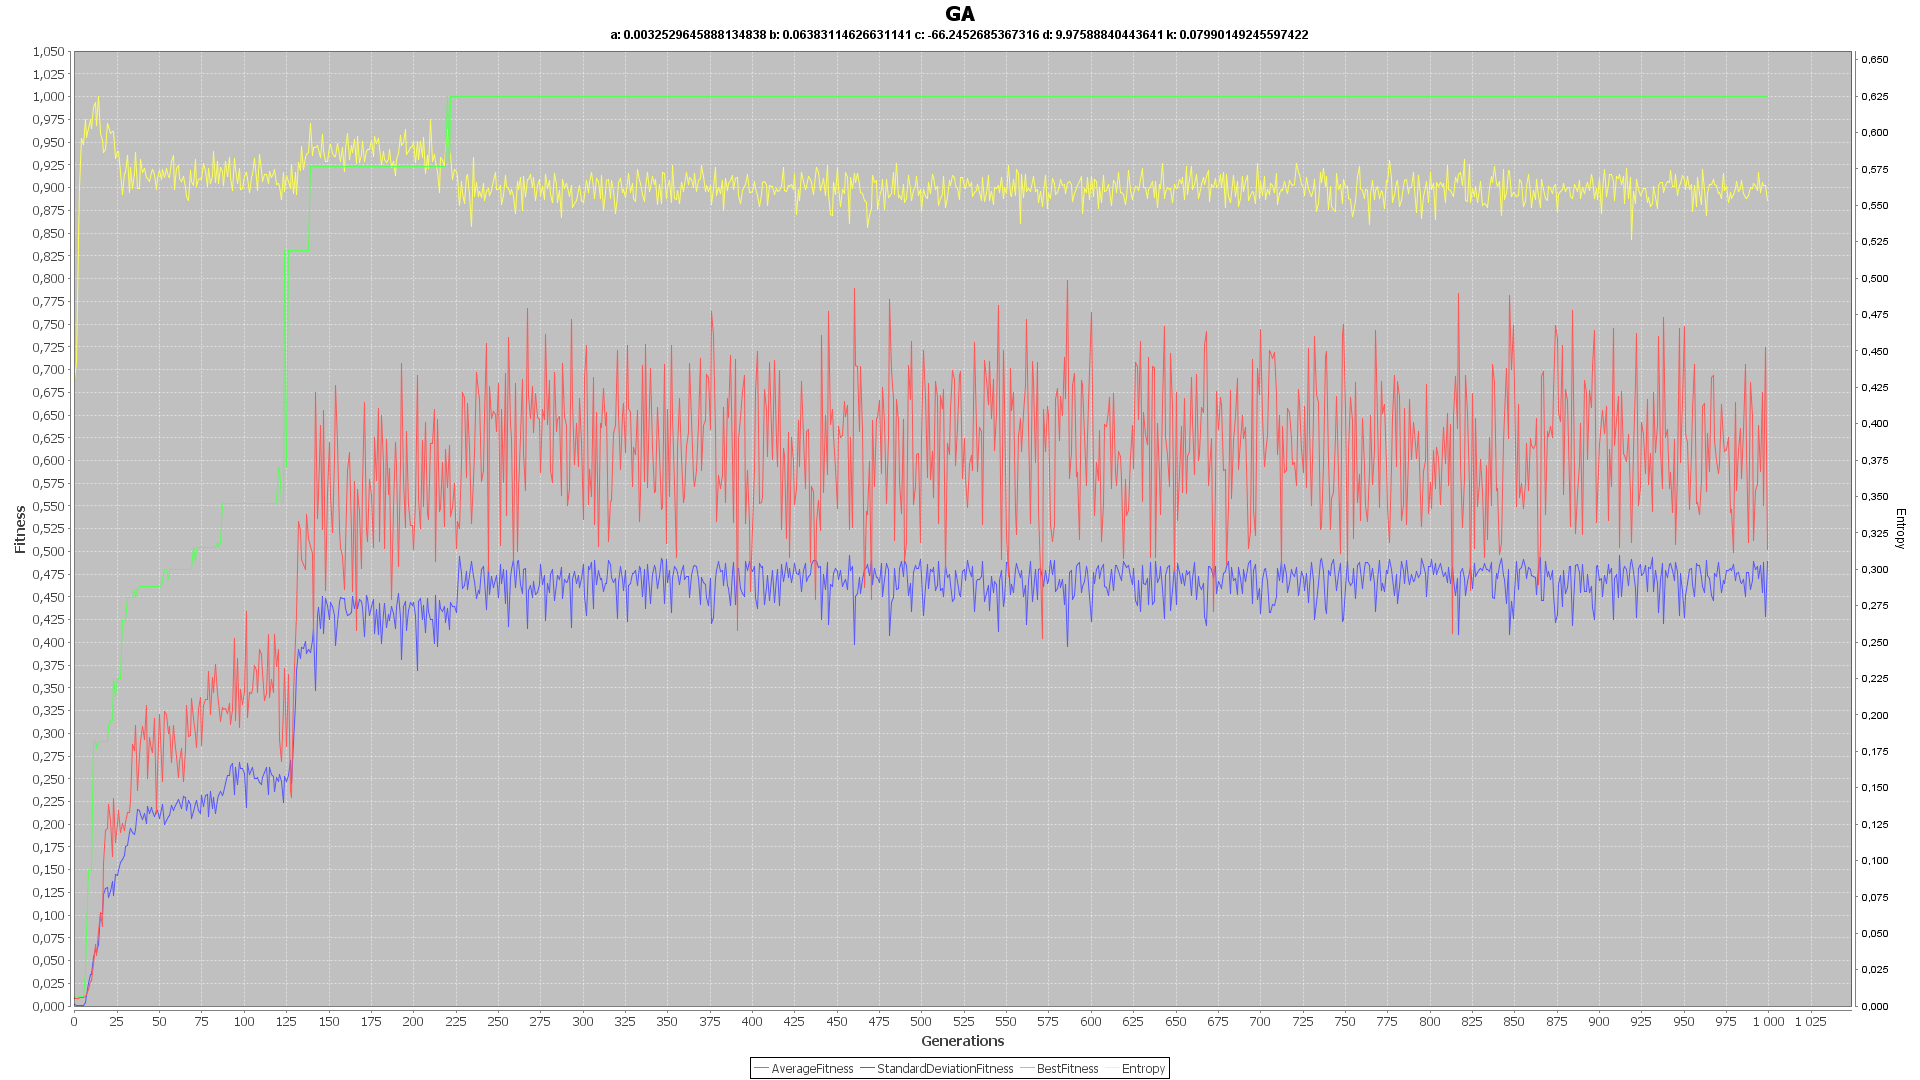
\includegraphics[width=\linewidth]{./../images/izzy4/time/prog.png}
						
						\label{fig:sub10b}
					\end{subfigure}
					
					\label{fig:plot10}
			\end{figure}
			
		\subsubsection{Spike interval distance metric}
			\begin{figure}[H]
				\centering
					\begin{subfigure}{.5\textwidth}
						\centering
						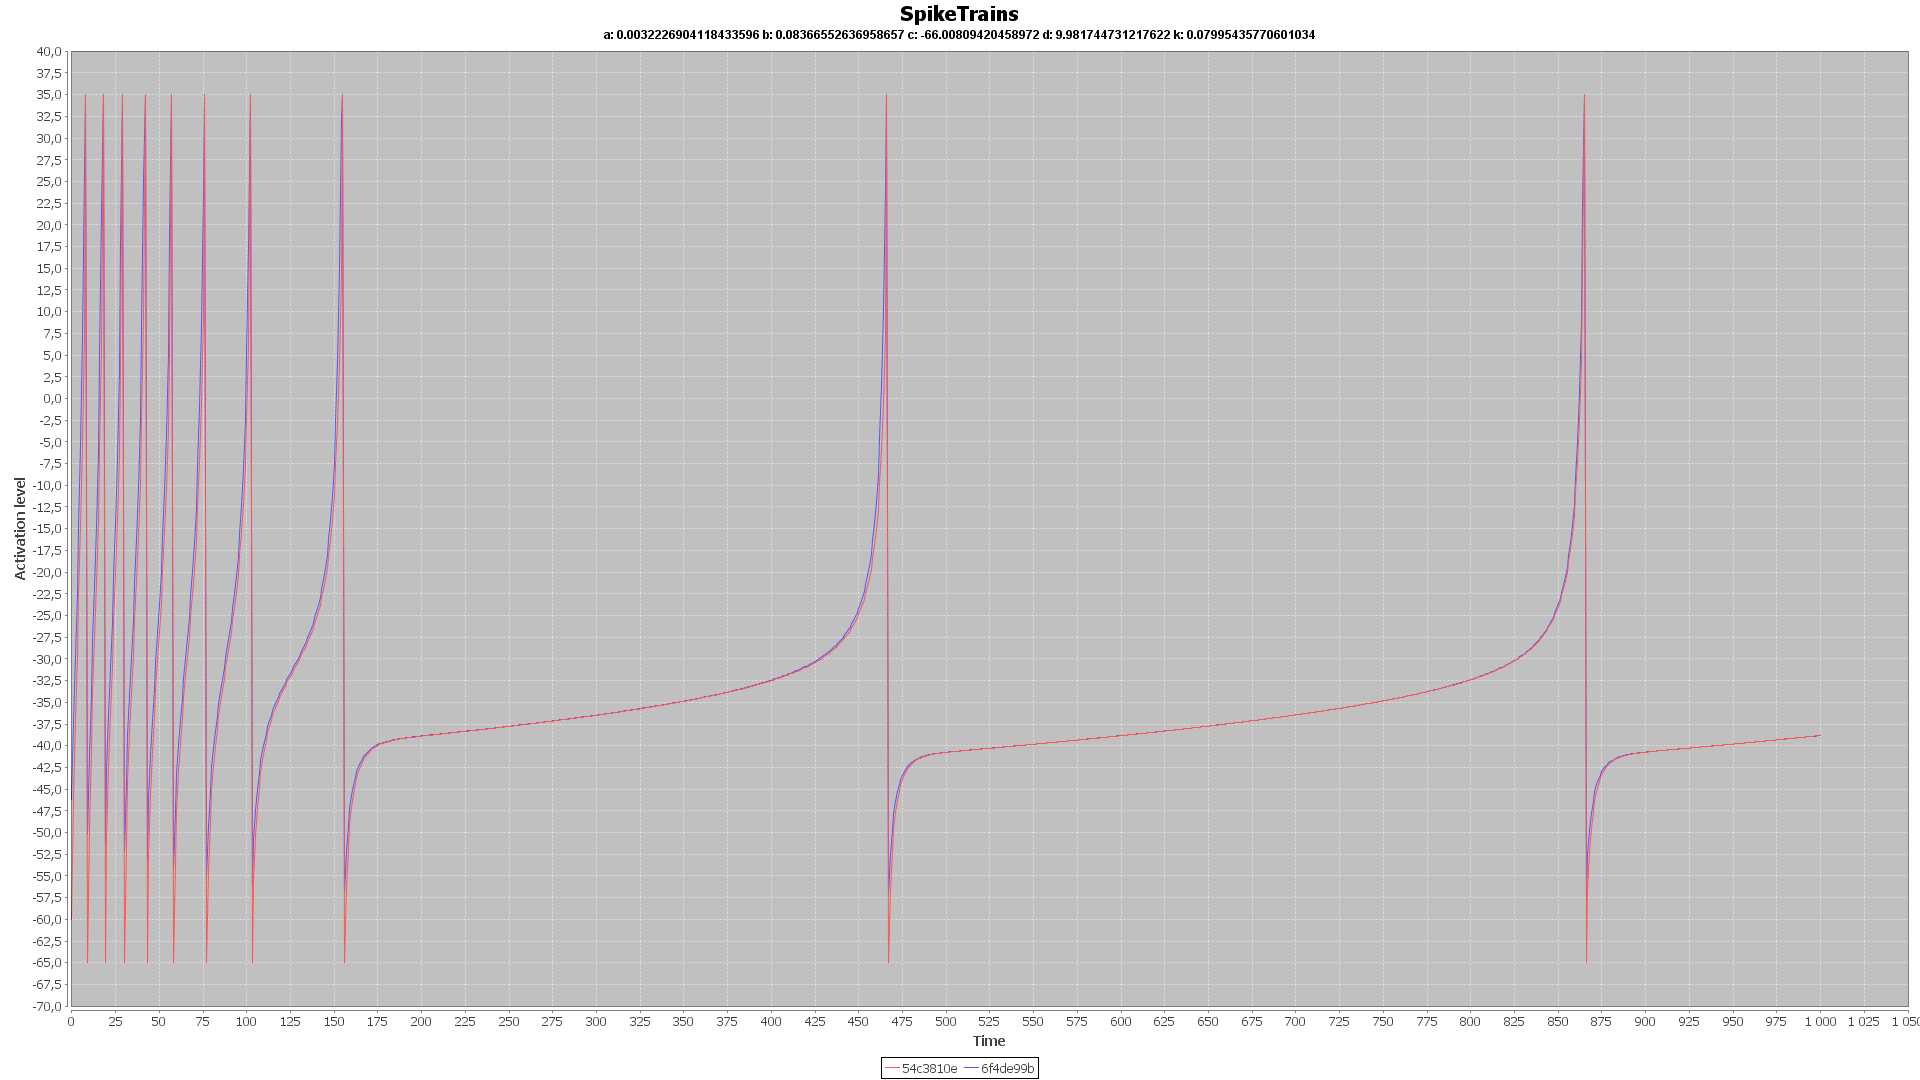
\includegraphics[width=\linewidth]{./../images/izzy4/interval/plot.png}
						
						\label{fig:sub11a}
					\end{subfigure}%
					\begin{subfigure}{.5\textwidth}
						\centering
						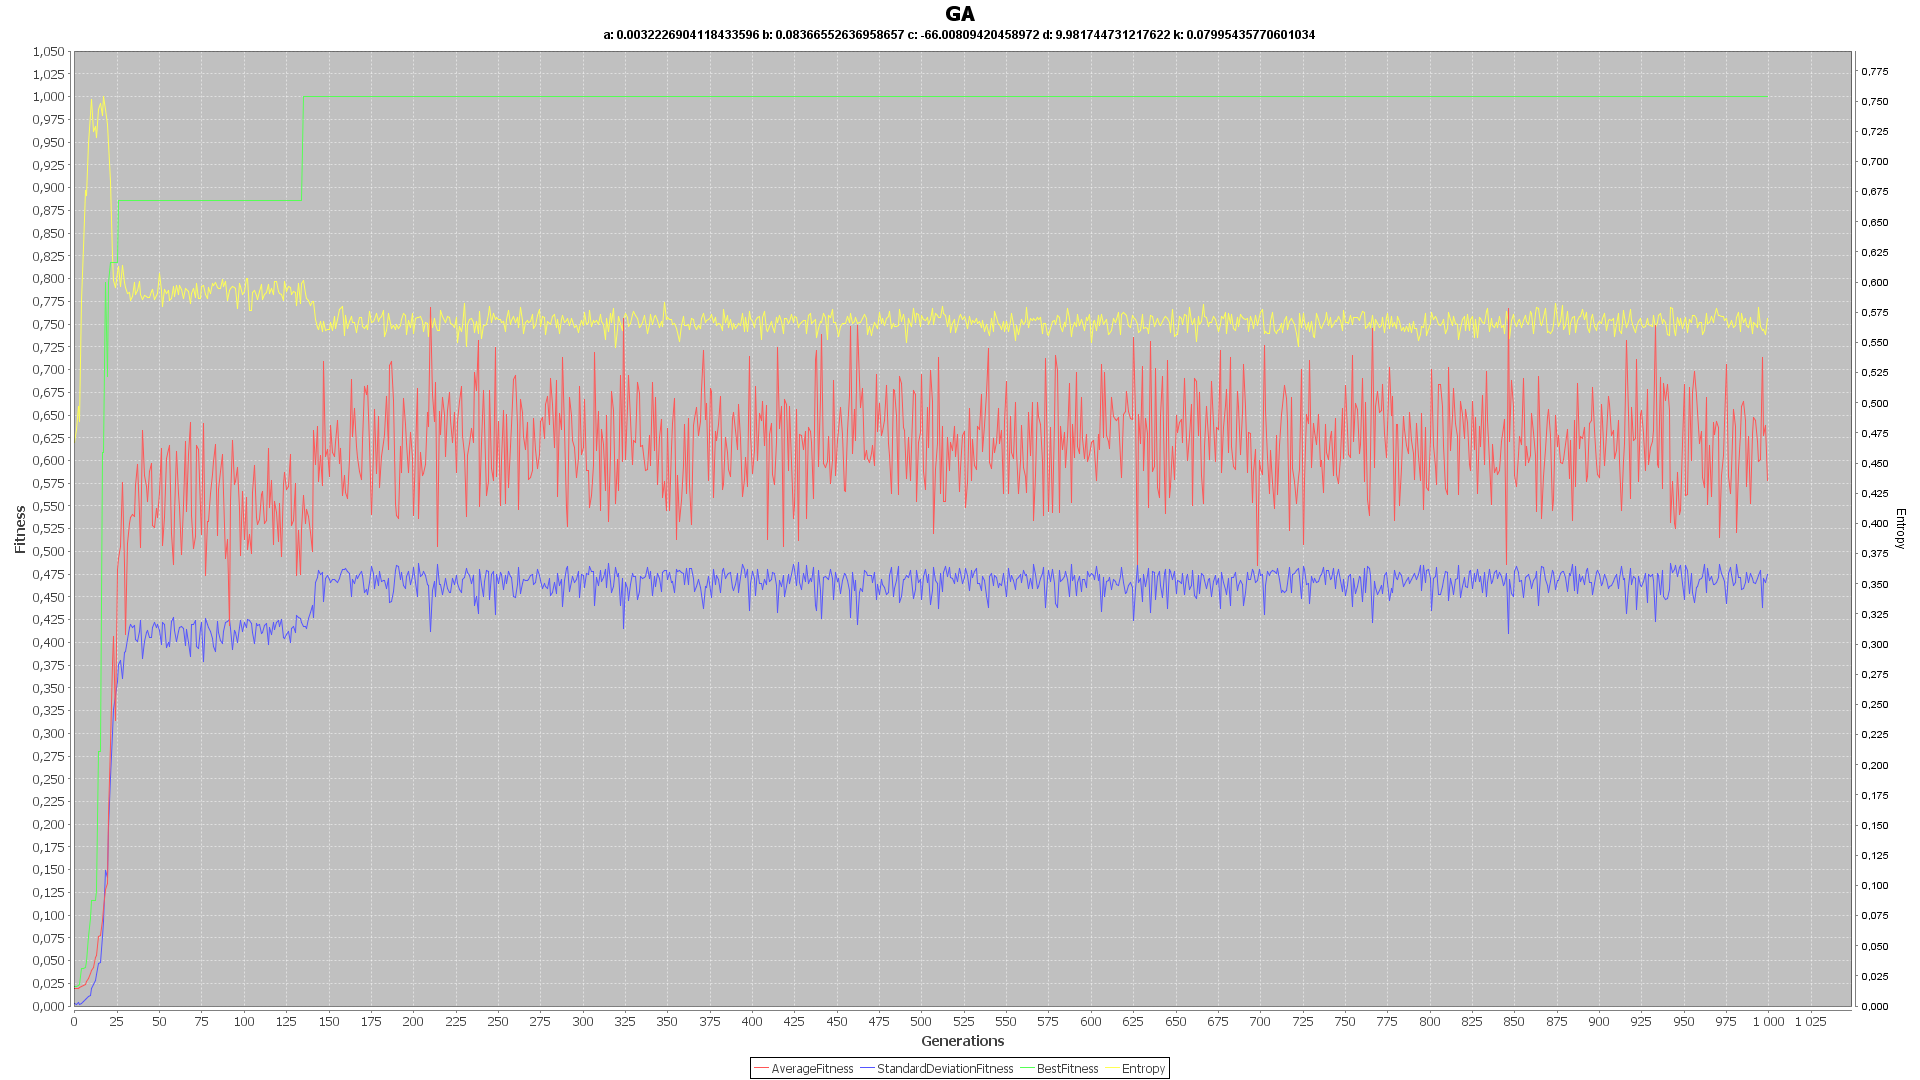
\includegraphics[width=\linewidth]{./../images/izzy4/interval/prog.png}
						
						\label{fig:sub11b}
					\end{subfigure}
					
					\label{fig:plot11}
			\end{figure}
		\subsubsection{Waveform distance metric}
	
\section{Genotype-Phenotype mapping}\label{sec:mapping}
In our implementation the genes in the genotype class encodes the parameters of the spiking neuron. The parameters are the ones who decidede how the spiking train progress as time goes by. The genes does not dictate the traits of the phenotypes directly, so we have an indirect mapping (more specifically the genotype-phenotype mapping is a generative (developmental) encoding scheme. This encoding scheme has the advantage of being good at scaling (large phenotypes can be created from compact phenotypes), and it's more biologically realistic. On the other hand, generative encoding has the disadvantage of having a hard time finding needle in a haystack optimal solutions.
\section{Practical implications}\label{sec:implications}
The program we have built accepts spike trains as input data and finds the best parameters to recreate them with the Izhikevich spiking-neuron model. The input may be any spike train, and our program will strive to find parameters to reproduce the same spike trains. This can be used by a proper neuroscientist, for instance if s/he registers actual signals from real neurons in a real brain, and input the into our program. The program output can be used to simulate neurons (which behaves like the real one) and use them in a computer simulation of the brain.
\section{Application in other problem domains}\label{sec:applications}
As mentioned in section \ref{sec:implications} our program finds the best parameters to create a neuron with the Izhikevich spiking-neuron model. It also measures the distance between our neuron and a target neuron, and tries to find a solution closer to the target. We can change our program by either allowing more distance metrics, change the way we measure fitness, or change the datarepresentation. The latter might be a way of generalizing the program: we could use different neurons, or perhaps a network of neurons, and use this to solve the traveling salesman problem.

The prerequisites for using our program to solve traveling salesman problems would first of all encompass the datarepresentation: how are the cities connected to each other, etc. We would also need a fitness function where shorter paths yields better results. See \ref{fig:fig1337} for a sketch of the overall system.
	\begin{figure}[H]
		\centering
			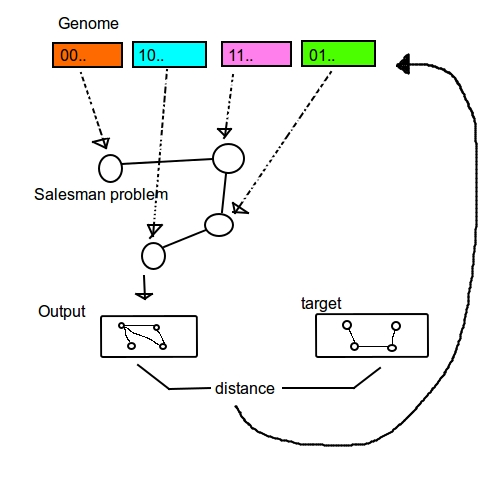
\includegraphics[width=0.5\linewidth]{./../images/sexyimage.jpg}
		\label{fig:fig1337}
	\end{figure}
\end{document}